\documentclass[11pt,a4paper]{article}
\usepackage[T1]{fontenc}
\usepackage[utf8]{inputenc}
\usepackage[sc]{mathpazo}
\linespread{1.04}
\usepackage[scaled=0.86]{helvet}
\usepackage[margin=1in]{geometry}
\usepackage{amsmath,amssymb,amsthm,mathtools}
\usepackage{booktabs}
\usepackage{array}
\usepackage{tabularx}
\usepackage{float}
\usepackage[hidelinks]{hyperref}
\usepackage[nameinlink,noabbrev]{cleveref}
\usepackage{microtype}
\usepackage{enumitem}
\usepackage{siunitx}
\usepackage{xcolor}
\usepackage{caption}
\usepackage{tcolorbox}
\tcbuselibrary{skins,breakable}
\usepackage{thmtools}
\usepackage{tikz}
\usetikzlibrary{arrows.meta,positioning,calc,fit,backgrounds,matrix,decorations.pathmorphing}
\usepackage{pgfplots}
\pgfplotsset{compat=1.18}
\usepackage{longtable}
\usepackage{multirow}
\usepackage{makecell}
\usepackage{bm}
\usepackage{csquotes}
\usepackage{fancyhdr}
\usepackage{titlesec}

% ── Color palette ──
\definecolor{tfptblue}{RGB}{35,60,120}
\definecolor{tfptorange}{RGB}{190,100,20}
\definecolor{tfptgreen}{RGB}{40,110,60}
\definecolor{tfptgray}{RGB}{90,90,95}

\hypersetup{
    colorlinks=true,
    linkcolor=tfptblue!80!black,
    citecolor=tfptblue!70!black,
    urlcolor=tfptblue!60!black,
}

% ── Caption styling ──
\captionsetup{
    font={small,sf},
    labelfont={bf,color=tfptgray},
    labelsep=period,
    margin=1.5em,
    skip=6pt,
}

% ── Section heading styling ──
\titleformat{\section}
    {\Large\bfseries\color{tfptblue}}{\thesection}{0.8em}{}
\titleformat{\subsection}
    {\large\bfseries\color{tfptblue!85!black}}{\thesubsection}{0.7em}{}
\titleformat{\subsubsection}
    {\normalsize\bfseries\color{tfptblue!70!black}}{\thesubsubsection}{0.6em}{}
\titlespacing*{\section}{0pt}{1.8ex plus 0.6ex minus 0.3ex}{0.9ex plus 0.2ex}
\titlespacing*{\subsection}{0pt}{1.4ex plus 0.4ex minus 0.2ex}{0.6ex plus 0.1ex}

% ── Running headers ──
\pagestyle{fancy}
\setlength{\headheight}{22pt}
\fancyhf{}
\fancyhead[L]{\small\itshape\color{tfptgray} TFPT 4.5: Boundary Polarization and Closed-Branch Dynamics}
\fancyhead[R]{\small\color{tfptgray}\thepage}
\renewcommand{\headrulewidth}{0.4pt}
\renewcommand{\headrule}{\hbox to\headwidth{\color{tfptblue!30}\leaders\hrule height \headrulewidth\hfill}}
\fancypagestyle{plain}{\fancyhf{}\fancyfoot[C]{\small\color{tfptgray}\thepage}\renewcommand{\headrulewidth}{0pt}}

% ── tcolorbox global defaults ──
\tcbset{
    enhanced,
    boxrule=0.6pt,
    arc=2.5pt,
    left=6pt, right=6pt, top=5pt, bottom=5pt,
    fonttitle=\bfseries\sffamily\small,
    coltitle=white,
    toptitle=2pt, bottomtitle=2pt,
    shadow={0.8mm}{-0.6mm}{0mm}{black!12},
}

\sisetup{
    detect-all,
    round-mode = none,
    exponent-mode = input,
    exponent-product = \times,
    group-separator = {\,},
    group-minimum-digits = 4
}

\newtheorem{theorem}{Theorem}[section]
\newtheorem{corollary}[theorem]{Corollary}
\newtheorem{lemma}[theorem]{Lemma}
\theoremstyle{definition}
\newtheorem{definition}[theorem]{Definition}
\newtheorem{conjecture}[theorem]{Conjecture}
\newtheorem{proposition}[theorem]{Proposition}
\newtheorem{assumption}[theorem]{Assumption}
\newtheorem{axiom}[theorem]{Axiom}
\newtheorem{principle}[theorem]{Principle}
\newtheorem{construction}[theorem]{Construction}
\newtheorem{claim}[theorem]{Claim}
\newtheorem{appendixstep}[theorem]{Appendix Step}
\theoremstyle{remark}
\newtheorem*{remark}{Remark}

\crefformat{thmt@dummyctr}{Remark}
\Crefformat{thmt@dummyctr}{Remark}
\crefname{thmt@dummyctr}{remark}{remarks}
\Crefname{thmt@dummyctr}{Remark}{Remarks}
\crefname{conjecture}{conjecture}{conjectures}
\Crefname{conjecture}{Conjecture}{Conjectures}
\crefname{definition}{definition}{definitions}
\Crefname{definition}{Definition}{Definitions}

\makeatletter
\def\theHtheorem{\thesection.\thetheorem}
\def\theHcorollary{\theHtheorem}
\def\theHlemma{\theHtheorem}
\def\theHdefinition{\theHtheorem}
\def\theHconjecture{\theHtheorem}
\def\theHproposition{\theHtheorem}
\def\theHassumption{\theHtheorem}
\def\theHprinciple{\theHtheorem}
\def\theHconstruction{\theHtheorem}
\def\theHclaim{\theHtheorem}
\def\theHappendixstep{\theHtheorem}
\makeatother

\DeclareMathOperator{\tr}{Tr}
\DeclareMathOperator{\rank}{rank}
\DeclareMathOperator{\SF}{SF}
\DeclareMathOperator{\Ind}{Ind}
\DeclareMathOperator{\argmin}{arg\,min}

\newcolumntype{Y}{>{\raggedright\arraybackslash}X}

\newcommand{\Seam}{\Sigma}
\newcommand{\inv}{\iota}
\newcommand{\taudbl}{\tau_{\mathrm{dbl}}}
\newcommand{\iC}{\iota_{\mathrm C}}
\newcommand{\epscar}{\varepsilon_{\mathrm{car}}}
\newcommand{\Xbulk}{X_{\mathrm{bulk}}}
\newcommand{\Mpl}{\bar M_{\mathrm{Pl}}}
\newcommand{\Mplunred}{M_{\mathrm{Pl}}}
\newcommand{\cthree}{c_3}
\newcommand{\atheta}{a_\theta}
\newcommand{\phibase}{\varphi_{\mathrm{base}}}
\newcommand{\phiz}{\varphi_0^{\mathrm{ret}}}
\newcommand{\phiseam}{\varphi_{\Sigma}}
\newcommand{\deltatop}{\delta_{\mathrm{top}}}
\newcommand{\omegaCCEW}{\omega_{\mathrm{CC}}^{(2)}}
\newcommand{\bone}{b_1}
\newcommand{\SM}{\mathrm{SM}}
\newcommand{\QCD}{\mathrm{QCD}}
\newcommand{\Oadm}{\Omega_{\mathrm{adm}}}
\newcommand{\Cmin}{\mathcal C_{\min}}
\newcommand{\Ageom}{\mathcal A_{\mathrm{geom}}}
\newcommand{\Atrans}{\mathcal A_{\mathrm{trans}}}
\newcommand{\Arec}{\mathcal A_{\mathrm{rec}}}
\newcommand{\Aobs}{\mathcal A_{\mathrm{obs}}}
\newcommand{\Asing}{\mathcal A_{\mathrm{sing}}}
\newcommand{\Vadm}{\mathcal V_{\mathrm{adm}}}
\newcommand{\Hrel}{\mathcal H_{\mathrm{rel}}}
\newcommand{\Hhad}{\mathcal H_{\mathrm{had}}}
\newcommand{\Hhub}{H_{\mathrm{hub}}}
\newcommand{\Htot}{\mathcal H_{\mathrm{tot}}}
\newcommand{\Gammaeff}{\Gamma_{\mathrm{eff}}}
\newcommand{\lambdaY}{\lambda_Y}
\newcommand{\Pred}{\operatorname{Pred}}
\newcommand{\gcar}{g_{\mathrm{car}}}
\newcommand{\Hint}{\mathcal H_{\mathrm{int}}}
\newcommand{\Kadm}{K_{\mathrm{adm}}}
\newcommand{\Tmin}{\mathfrak T_{\mathrm{min}}}
\newcommand{\Tbound}{\mathfrak T_{\partial}^{\min}}
\newcommand{\Tprim}{\mathfrak T_{\mathrm{prim}}}
\newcommand{\chiseed}{\chi_{\mathrm{seed}}}
\newcommand{\chigeo}{\chi_{\mathrm{geo}}}
\newcommand{\chigeozero}{\chi_{\mathrm{geo},0}}
\newcommand{\APSdom}{\mathrm{APS}_{\mathrm{dom}}}
\newcommand{\APSfam}{\mathrm{APS}_{\mathrm{fam}}}
\newcommand{\vgeo}{v_{\mathrm{geo}}}
\newcommand{\vewref}{v_{\mathrm{EW}}^{\mathrm{ref}}}
\newcommand{\Dstart}{D_{\mathrm{start}}}
\newcommand{\Tcore}{\mathfrak T_{\mathrm{core}}}
\newcommand{\Tbridge}{\mathfrak T_{\mathrm{bridge}}}
\newcommand{\Tker}{\mathfrak T_{\mathrm{ker}}}
\newcommand{\Tcomp}{\mathfrak T_{\mathrm{comp}}}
\newcommand{\Padm}{P_{\mathrm{adm}}}
\newcommand{\Pprim}{P_{\mathrm{prim}}}
\newcommand{\Tpre}{\mathfrak T_{\mathrm{pre}}}
\newcommand{\Tstar}{\mathfrak T_{\star}}
\newcommand{\APSdomprov}{\mathrm{APS}_{\mathrm{dom}}^{\mathrm{prov}}}
\newcommand{\sigmaQCD}{\sigma_{\mathrm{QCD}}}
\newcommand{\Cseam}{\mathcal C_{\Sigma}}
\newcommand{\Ccyc}{\mathfrak C_{\Sigma}}
\newcommand{\Ffals}{\mathsf F_{\mathrm{fals}}}
\newcommand{\Rcmp}{\mathcal R_{\mathrm{cmp}}}
\newcommand{\wspin}{\varpi_{\mathrm{spin}}}
\newcommand{\PhysAdmOne}{\widehat{\mathrm{PhysAdm}}_1}
\newcommand{\ObsAdm}{\mathbf{Obs}_{\mathrm{adm}}}
\newcommand{\GrenTFPT}{\Gamma_{\mathrm{TFPT}}^{\mathrm{ren}}}
\newcommand{\OphysTFPT}{\mathbf O_{\mathrm{phys}}^{\mathrm{TFPT}}}
\newcommand{\OschemeTFPT}{\mathbf O_{\mathrm{scheme}}^{\mathrm{TFPT}}}
\newcommand{\SchGrp}{\mathbf{Sch}}
\newcommand{\Runiv}{\mathfrak R}
\newcommand{\Mop}{\mathfrak M}
\newcommand{\Mphys}{\mathfrak M_{\mathrm{phys}}}
\newcommand{\Mscheme}{\mathfrak M_{\mathrm{scheme}}}
\newcommand{\Rren}{\mathfrak R_{\mathrm{ren}}}
\newcommand{\Bind}{\mathcal B_{\mathrm{ind}}}
\newcommand{\Clrig}{\mathfrak{Cl}}
\newcommand{\Runivrig}{\overline{\Runiv}}
\newcommand{\Seedop}{\mathbf{Seed}^{\mathrm{op}}}
\newcommand{\Cseed}{\mathfrak C_{\mathrm{seed}}}
\newcommand{\triv}{\textup{triv}}
\newcommand{\rankess}{\rank_{\textup{ess}}}
\newcommand{\red}{\textup{red}}


% -- TFPT 4.5 split helpers --
\newcommand{\sourceDraft}{\texttt{../tfpt-42.tex}}
\newcommand{\paperstatus}{Draft split from \sourceDraft; theorem wording still inherits the status discipline of the source manuscript.}

\newenvironment{tfptfrontbox}
{\begin{tcolorbox}[colback=tfptblue!2, colframe=tfptblue!45, breakable,
    title={Scope box: inputs, contribution, non-claims, audit surface}, colbacktitle=tfptblue!65]}
{\end{tcolorbox}}

\newenvironment{tfptwarningbox}
{\begin{tcolorbox}[colback=tfptorange!4, colframe=tfptorange!55, breakable,
    title={Editorial guardrail}, colbacktitle=tfptorange!75]}
{\end{tcolorbox}}

\newenvironment{tfptsourcebox}
{\begin{tcolorbox}[colback=tfptgreen!3, colframe=tfptgreen!50, breakable,
    title={Source extraction map}, colbacktitle=tfptgreen!65]}
{\end{tcolorbox}}

\newcommand{\TFPTxref}[1]{\textup{[TFPT cross-reference: \texttt{\detokenize{#1}}]}}
\newcommand{\TFPTeqref}[1]{\textup{[TFPT equation: \texttt{\detokenize{#1}}]}}

\newenvironment{tfptclaimcontract}
{\begin{tcolorbox}[colback=tfptblue!2, colframe=tfptblue!50, breakable,
    title={Claim contract}, colbacktitle=tfptblue!70]\small}
{\end{tcolorbox}}

\newenvironment{tfptexports}
{\begin{tcolorbox}[colback=tfptgreen!3, colframe=tfptgreen!50, breakable,
    title={Exported objects}, colbacktitle=tfptgreen!65]}
{\end{tcolorbox}}



\title{\color{tfptblue}\textbf{Admissibility, Strong CP, and Nonperturbative QFT Closure}\\[0.35em]
{\Large on the TFPT Branch}}
\author{Stefan Hamann \and Alessandro Rizzo}
\date{{\normalsize\color{tfptgray}\sffamily Paper 4 of the TFPT 4.5 series -- \today}}

\begin{document}
\maketitle

\begin{abstract}
This paper isolates the analytic closure layer of TFPT. The selector $\Padm$ is treated as a
physical admissible-sector construction, while the dynamics is carried by $Z_{\mathrm{rel}}$,
admissible Schwinger distributions, Osterwalder--Schrader reconstruction, the local Minkowski net,
stable massive scattering, and the exact admissible RG flow.
\end{abstract}

\begin{tfptfrontbox}
\textbf{Inputs from previous papers.} Paper 1 supplies $\Pprim$. Paper 2 supplies the carrier and
discrete determinant data needed for $P_{\mathrm{sing}}$ and $P_\Theta$. Paper 3 is not logically
required except for optional observable cross-references.

\textbf{New theorem contribution.} Conditional nonperturbative closure on the admissible sector:
\[
\Padm=\Pprim P_{\mathrm{sing}}P_\Theta,\qquad
\theta_{\mathrm{eff}}=0,\qquad
\operatorname{arg}\det M_u=\operatorname{arg}\det M_d=0,
\]
together with reflection positivity, OS reconstruction, local Minkowski net, stable massive
scattering, and exact admissible flow.

\textbf{Not claimed here.} No $\alpha$ detail calculation, no CMB, no E8, and no full empirical
tables.

\textbf{Falsification or audit surface.} The paper fails if selector and dynamics are conflated, if
positivity/gap hypotheses are hidden, or if strong-CP closure uses an inadmissible phase convention.
\end{tfptfrontbox}

\begin{tfptwarningbox}
Preferred claim language: \emph{conditional nonperturbative closure under explicitly stated
admissibility, positivity, and gap hypotheses}. Avoid unqualified ``proved QFT'' rhetoric.
\end{tfptwarningbox}

\begin{tfptwarningbox}
Every analytic theorem in this paper is to be read with its hypotheses in the statement, not as an
unconditional construction of four-dimensional QFT. The standing checklist is: admissible
Schwinger family, temperedness, Euclidean covariance, reflection positivity, clustering,
locality-domain regularity, and a stated massive-sector gap where scattering is invoked.
\end{tfptwarningbox}


\begin{tfptclaimcontract}
\textbf{Claim.} $\Padm$ selects the physical sector; strong CP closes; QFT reconstruction is conditional on stated analytic hypotheses.\par
\textbf{Inputs.} $\Pprim$, carrier/determinant data, admissibility complex, positivity/gap hypotheses.\par
\textbf{First assumptions.} Reflection positivity, temperedness, Euclidean covariance, clustering, locality-domain regularity, sector gap.\par
\textbf{Proof status.} Conditional nonperturbative closure / standard-theorem interface.\par
\textbf{Kill condition.} Hidden positivity/gap assumption, nonzero strong-CP angle, or failure of OS/local-net hypotheses.\par
\end{tfptclaimcontract}

\tableofcontents

\section{Selector Versus Dynamics}

The central distinction is
\[
\Padm\quad\text{selects the physical sector},
\]
whereas dynamics is carried by
\[
Z_{\mathrm{rel}}
\Rightarrow
\{S_n^T\}
\Rightarrow
(\mathcal H_{\mathrm{adm}},\mathfrak A_{\mathrm{adm}})
\Rightarrow
\Gamma_k
\Rightarrow
\GrenTFPT .
\]
This separation must be repeated in the introduction and conclusion because it is the main defense
against overclaiming.

\section{Full Admissibility Complex}

After carrier and determinant data are fixed, the full selector is
\[
\Padm=\Pprim P_{\mathrm{sing}}P_\Theta.
\]
The paper should retain the two-stage upgrade from $\Pprim$ to $\Padm$, the Hodge projector
description, and the exact role of the gap projection. Carrier material is summarized only as an
input.

\section{Strong CP Closure}

The strong-CP sector is stated as an admissibility result:
\[
\theta_{\mathrm{eff}}=0,
\qquad
\operatorname{arg}\det M_u=0,
\qquad
\operatorname{arg}\det M_d=0.
\]
The argument should connect hadronic singlet selection, determinant structure,
$\gamma_5$-Hermiticity, and the sheet involution without importing phenomenological tuning.

\section{Reflection Positivity and OS Reconstruction}

The reflection-positivity block should state all assumptions on the admissible Schwinger functions,
fermionic positivity, quotient form, and domain regularity. The OS theorem is used as a standard
interface only after the admissible-sector positivity hypotheses are named.

\section{Local Net and Scattering}

The local Minkowski net, Haag--Ruelle/LSZ massive scattering, and dressed massless interface are
treated as conditional closure outputs. The paper must distinguish stable massive scattering from
low-curvature dressed massless behavior.

\section{Exact Admissible Flow}

The exact admissible RG flow is the analytic continuation of the same sector:
\[
\partial_k\Gamma_k
=
\frac12\operatorname{STr}\left[(\Gamma_k^{(2)}+R_k)^{-1}\partial_kR_k\right]_{\mathrm{adm}},
\]
with the admissible projection included as part of the flow definition. The observable hierarchy is
included only as far as it supports the QFT closure layer.

\clearpage
\section{Main Technical Development}

This section contains the main technical development assigned to this paper by the TFPT 4.5 clean split. Cross-paper background is referenced through dependency and scope boxes; extended backend material is kept in the Technical Companion.

% Auto-extracted from ../tfpt-42.tex for the TFPT 4.5 clean split.
% Source body assigned by the TFPT 4.5 clean split.

% ---- Hadronic admissibility and strong-CP ingredients: source lines 7157-7357 ----
\subsection{Hadronic admissibility as singlet selection}

\begin{proposition}[Admissible color words]
For each carrier word $w$, let $z(w)\in\{1,\omega,\omega^2\}$ be its color-center charge and let $\varepsilon(w)\in\{\pm1\}$ be its seam parity. Physical hadronic words satisfy
\[
z(w)=1,
\qquad
\varepsilon(w)=+1.
\]
\end{proposition}

This is a superselection statement on the retained branch, not a derivation of dynamical confinement from the microscopic Yang--Mills flow. The corresponding hadronic Hilbert space will be written explicitly in \TFPTxref{sec:closure-theorems}. A schematic version is shown in \Cref{fig:admissible-words}.

\begin{figure}[t]
\centering
\begin{tikzpicture}[>=Latex, node distance=1.1cm and 1.3cm]
\node[draw=red!70!black, fill=red!4, rounded corners, minimum width=2.1cm, minimum height=1.0cm, align=center] (q) {free quark\\$z(w)\neq 1$};
\node[draw=green!50!black, fill=green!4, rounded corners, minimum width=2.1cm, minimum height=1.0cm, align=center, right=of q] (m) {meson\\$z(w)=1$};
\node[draw=green!50!black, fill=green!4, rounded corners, minimum width=2.1cm, minimum height=1.0cm, align=center, right=of m] (b) {baryon\\$z(w)=1$};
\draw[red!70!black, very thick] ($(q.north west)+(0.12,-0.12)$) -- ($(q.south east)+(-0.12,0.12)$);
\draw[red!70!black, very thick] ($(q.south west)+(0.12,0.12)$) -- ($(q.north east)+(-0.12,-0.12)$);
\node[below=0.2cm of q] {\small excluded};
\node[below=0.2cm of m] {\small admissible};
\node[below=0.2cm of b] {\small admissible};
\end{tikzpicture}
\caption{Hadronic admissibility as singlet selection.}
\label{fig:admissible-words}
\end{figure}

The transport-sector QCD string tension is written as
\[
\sigmaQCD=\cthree^2\chi_{\QCD}^2,
\]
so the relative Wilson loop obeys
\[
\langle W(C)\rangle_{\mathrm{rel}}\sim e^{-\sigmaQCD A(C)}.
\]
Throughout the manuscript we write $\sigmaQCD$ explicitly for the QCD string tension to keep
it lexically distinct from the local Weyl conformal factor $\sigma$ of the geometric branch and
from the standard-deviation $\sigma$ used in benchmark tables. The sector-dependent scale
$\chi_{\QCD}$ is the minimal notation needed to avoid confusing the hadronic transport channel
with the gravitational $\chigeozero$ background; the two channels are linked by the common
underlying primitive response $\chiseed$ but not by a naive equality of scales.

\subsection{Transport-side ingredients for the strong-CP sector}

Define
\begin{equation}
\label{eq:strong-cp}
\bar\theta=\theta_{\mathrm{QCD}}+\arg\det M_u+\arg\det M_d.
\end{equation}
\begin{definition}[Sheet-CP symmetry on the admissible branch]
\label{def:sheet-cp-symmetry}
Define the admissible sheet-CP operator by
\[
\mathcal C_\Sigma:=CP\circ\taudbl.
\]
\end{definition}

\begin{theorem}[Determinant-line phase and strong-CP seed on the admissible branch]
\label{thm:sheet-cp-protection}
\label{thm:structural-strong-cp}
On the closed branch the hard holonomy factorization gives, for $f=u,d$,
\[
Y_f=D_{L,f}U_f^\star D_{R,f},
\qquad
\;D_{L,f},D_{R,f}>0,
\qquad
U_f^\star\in SU(3)_F.
\]
For
\[
M_f=\frac{\vgeo}{\sqrt2}Y_f
\]
one has
\[
\det M_f>0,
\qquad
\arg\det M_u=\arg\det M_d=0.
\]
Moreover the polar unitary factor
\[
U_f^{\mathrm{pol}}:=M_f(M_f^\dagger M_f)^{-1/2}
\]
lies in $SU(3)_F$. The antiunitary sheet operation
preserves the admissible relative action $\Gamma_{\mathrm{rel}}$:
\[
\mathcal C_\Sigma\,\Gamma_{\mathrm{rel}}\,\mathcal C_\Sigma^{-1}=\Gamma_{\mathrm{rel}},
\qquad
\mathcal C_\Sigma\,Q\,\mathcal C_\Sigma^{-1}=-Q,
\]
so the sheet operation acts as a stability symmetry of the same branch. The same admissible seam
operator determines the canonical determinant-line phase
\[
a_\Sigma:=\arg\det_{\mathrm{adm}}U_\Sigma\in S^1_{\det},
\]
whose canonical winding is inherited from the unit boundary winding of the seam class. Weak CP may
still survive through
\[
V_{\mathrm{CKM}}=U_{u,L}^\dagger U_{d,L}.
\]
\end{theorem}

\begin{proof}
From the hard holonomy factorization one gets
\[
\det M_f
=
\left(\frac{\vgeo}{\sqrt2}\right)^3
\det D_{L,f}\det D_{R,f}\det U_f^\star
>
0,
\]
because the diagonal factors are positive and $\det U_f^\star=1$. Hence
\[
\arg\det M_f=0.
\]
Equivalently, in any admissible biunitary polar form
\[
M_f=U_{f,L}H_fU_{f,R}^\dagger,
\qquad
H_f>0,
\qquad
U_{f,L},U_{f,R}\in SU(3)_F,
\]
the spectral theorem gives $\det H_f>0$ and therefore
\[
\det M_f=\det(U_{f,L})\det(H_f)\overline{\det(U_{f,R})}=\det H_f>0,
\]
so the same determinant-phase suppression follows directly from $\det H_f>0$ and
$\det U_{f,L}=\det U_{f,R}=1$.
For the polar unitary factor one has
\[
\det U_f^{\mathrm{pol}}
=
\frac{\det M_f}{|\det M_f|}
=
1,
\]
so $U_f^{\mathrm{pol}}\in SU(3)_F$. Independently, the deck involution $\taudbl$
implements sheet exchange on the admissible branch, so composing it with $CP$ yields an exact
antiunitary symmetry of the relative action while flipping the sign of the topological charge.
This shows that the sheet operation stabilizes the branch already selected by the determinant
structure, rather than generating the vanishing from scratch. The same seam operator already
carries a canonical determinant-line phase, and unit seam spectral flow upgrades that phase to the
natural compact strong-CP angle variable of the branch. Weak CP may still survive through a
nontrivial Jarlskog invariant in the relative family holonomies.
\end{proof}

\begin{corollary}[RG and matching invariance of determinant-phase suppression]
\label{cor:strong-cp-rg-stability}
In every renormalization scheme that respects $\Cseam$, $\Padm$, and the carrier structure, the
determinant-phase suppression
\[
\arg\det M_u=\arg\det M_d=0
\]
of \TFPTxref{thm:sheet-cp-protection} is preserved under the declared RG flow and matching map.
The same determinant-line phase $a_\Sigma$ remains scheme-stable, so the structural input to
\Cref{thm:strong-cp-closure} survives RG flow as well.
\end{corollary}

\begin{lemma}[Retained-branch \texorpdfstring{$\gamma_5$}{gamma5}-Hermiticity]
\label{lem:retained-gamma5-hermiticity}
For each quark sector $f=u,d$, let $D_{E,f}$ be the Euclidean kinetic Dirac operator on the
admissible branch and define
\[
\mathcal D_f:=D_{E,f}+M_fP_R+M_f^\dagger P_L,
\qquad
P_{L,R}:=\frac{1\mp\gamma_5}{2}.
\]
Then
\[
\mathcal D_f^\dagger=\gamma_5\mathcal D_f\gamma_5.
\]
\end{lemma}

\begin{proof}
The Euclidean kinetic operator is anti-Hermitian and anticommutes with $\gamma_5$. The mass block
on the admissible branch is the positive polar mass map of \TFPTxref{thm:sheet-cp-protection}, hence
enters as the Hermitian chiral pair $M_fP_R+M_f^\dagger P_L$. The displayed identity follows
immediately.
\end{proof}

The positive-branch clause is still essential here: the closure statement is about the physical
mass map once the admissible transport branch has been fixed, not about an arbitrary unitary
dressing of the same singular values. What changes in the present rewrite is the logical source
of the null result: the branch no longer relies on a promise not to insert a bad counterterm by
hand, but on the polar structure first, the determinant line second, and the antiunitary sheet
symmetry third. The later strong-CP theorem closes the effective angle by combining exactly these
three ingredients with vacuum positivity.

\begin{remark}[Admissibility as a unified three-sector motif]
The admissibility pair $(\mathsf{Adm},\Padm)$ acts as a single structural principle with three sector projections:
\begin{itemize}[leftmargin=1.5em, topsep=3pt, itemsep=2pt]
    \item \textbf{Electroweak:} seam-even selection picks the unique light Higgs doublet ($\taudbl^{\ast}\Phi=+\Phi$).
    \item \textbf{QCD:} center neutrality selects confined hadronic words ($z(w)=1$, $\varepsilon(w)=+1$).
    \item \textbf{Strong CP:} the determinant structure, $\gamma_5$-Hermiticity, and the sheet involution close the strong angle internally on the admissible branch.
\end{itemize}
These are not three independent rules bolted onto different sectors. They are three projections of the same admissible-versus-inadmissible boundary: seam parity, center charge, and sheet exchange are all encoded in the double-cover and involution data of the primitive core. This unification is the conceptual backbone of the transport program.
\end{remark}


% ---- Closure theorems from the admissibility complex: source lines 7358-8906 ----
\section{Closure theorems from the admissibility complex}
\label{sec:closure-theorems}

The preceding two sections introduced the carrier-compatible geometric and transport architecture.
The primitive admissibility projector $\Pprim$ was already placed in the primitive section so
that the proof direction runs from the boundary datum through the derived closed datum to $\Pprim$, and only then to the later
sector theorems. What remains in this section is therefore (i) the upgrade of $\Pprim$ to the
full admissibility projector $\Padm$ once the discrete carrier and determinant data have been
fixed, and (ii) the closure stack that follows from that full projector together with the family,
Higgs, positivity, and reflection-stability inputs collected first.

\begin{definition}[Full admissibility complex]
\label{def:full-admissibility-complex}
Once the discrete carrier and determinant data are fixed on the admissible branch, the Hilbert
space carries a color factor and a determinant involution. Write
\[
\mathcal H=\mathcal H_{\Seam}\otimes\mathcal H_c\otimes\mathcal H_\Theta\otimes\mathcal H_t,
\qquad
\mathcal H_{\mathrm{ext}}
:=
\mathcal H\otimes\Lambda(\eta_\Sigma,\eta_c,\eta_\Theta,\eta_g),
\]
with carrier-side color generator $Z_c$ and determinant-sector involution $Q_\Theta$ satisfying
\[
\iC^2=\mathbf 1,
\qquad
Q_\Theta^2=\mathbf 1,
\qquad
Q_\Theta^\dagger=Q_\Theta.
\]
Define the full structural selector
\[
P_{\mathrm{str}}:=P_{\Seam,+}P_{\mathrm{sing}}P_\Theta,
\qquad
P_{\Seam,+}:=\frac{\mathbf 1+\iC}{2},
\qquad
P_\Theta:=\frac12(\mathbf 1+Q_\Theta),
\]
\[
P_{\mathrm{sing}}:=\frac13(\mathbf 1+Z_c+Z_c^2).
\]
Let $\epsilon_{\mathrm{adm}}>0$ and let $D_{\mathrm{adm}}$ be the admissible sector operator on
$\mathrm{Ran}(P_{\mathrm{str}})$ commuting with $\iC$, $P_{\mathrm{sing}}$, and $Q_\Theta$.
Define the elementary penalties
\[
K_\Sigma:=\sqrt{\lambda_\Sigma}\,\frac{\mathbf 1-\iC}{2},
\qquad
K_c:=\sqrt{\lambda_c}\,\bigl(\mathbf 1-P_{\mathrm{sing}}\bigr),
\]
\[
K_\Theta:=\sqrt{\lambda_\Theta}\,\frac{\mathbf 1-Q_\Theta}{2},
\qquad
K_g:=\sqrt{\lambda_{\mathrm{gap}}}\,\mathbf 1_{[0,\epsilon_{\mathrm{adm}}^2/4)}\!\bigl(P_{\mathrm{str}}D_{\mathrm{adm}}^\dagger D_{\mathrm{adm}}P_{\mathrm{str}}\bigr).
\]
The full admissibility differential is
\[
Q_{\mathrm{adm}}
:=
\eta_\Sigma^\dagger K_\Sigma
+\eta_c^\dagger K_c
+\eta_\Theta^\dagger K_\Theta
+\eta_g^\dagger K_g,
\]
and the full admissibility Laplacian is
\[
\Delta_{\mathrm{adm}}:=\{Q_{\mathrm{adm}},Q_{\mathrm{adm}}^\dagger\}.
\]
\end{definition}

\begin{theorem}[Two-stage upgrade from $\Pprim$ to $\Padm$]
\label{thm:padm-upgrade}
On the closed branch obtained after the carrier theorem and the compact bosonic index closure,
\[
Q_{\mathrm{adm}}^2=0,
\qquad
\Delta_{\mathrm{adm}}=K_\Sigma^2+K_c^2+K_\Theta^2+K_g^2=\Kadm,
\]
and the full Hodge projector
\[
\Padm
:=
\Pi_{\ker\Delta_{\mathrm{adm}}}
=
\operatorname*{s-lim}_{\beta\to\infty}e^{-\beta\Kadm}
\]
admits the two-stage factorization
\[
\Padm
=
\Pprim\,P_{\mathrm{sing}}\,P_\Theta
=
P_{\mathrm{str}}\,P_{\mathrm{gap}},
\qquad
P_{\mathrm{gap}}
:=
\mathbf 1_{[\epsilon_{\mathrm{adm}}^2/4,\infty)}\!\bigl(P_{\mathrm{str}}D_{\mathrm{adm}}^\dagger D_{\mathrm{adm}}P_{\mathrm{str}}\bigr).
\]
The first factor $\Pprim$ depends only on the primitive datum
$(\iC,\APSdom,D_{\mathrm{rel}})$; the second factor $P_{\mathrm{sing}}P_\Theta$ depends only on
the carrier and determinant data made available by the carrier and bosonic index theorems.
\end{theorem}

\begin{proof}[Proof sketch]
The auxiliary generators $\eta_\Sigma^\dagger,\eta_c^\dagger,\eta_\Theta^\dagger,\eta_g^\dagger$
anticommute, so $Q_{\mathrm{adm}}^2$ reduces to the commutators of $K_\Sigma,K_c,K_\Theta,K_g$.
The four commuting sectors $\mathcal H_\Seam,\mathcal H_c,\mathcal H_\Theta,\mathcal H_t$ are
acted on independently by these penalties, hence the mixed terms vanish and $\Delta_{\mathrm{adm}}=\Kadm$. The strong-coupling limit therefore projects onto the harmonic
admissible sector. Because $K_\Sigma$ and $K_g$ already define $\Pprim$ on
$\mathcal H_{\mathrm{prim}}$ and the additional penalties $K_c,K_\Theta$ commute with both, the
full projector factorizes through $\Pprim$ multiplicatively, giving the two-stage form.
\end{proof}

\begin{corollary}[Factorized selector as a derived form]
\label{cor:factorized-admissibility-selector}
On the admissible branch the familiar factorized selector
\[
\Padm=P_{\Seam,+}P_{\mathrm{sing}}P_\Theta\,P_{\mathrm{gap}}
\]
is recovered as a corollary of \TFPTxref{thm:padm-upgrade}; nothing in the primitive section depends
on it.
\end{corollary}

The two-stage selector geometry is summarized in \Cref{fig:admissibility-stack}.

\begin{figure}[t]
\centering
\scriptsize
\begin{tikzpicture}[
    >=Latex,
    data/.style={draw=black!60, fill=gray!8, rounded corners, text width=2.55cm, minimum height=0.9cm, align=center},
    prim/.style={draw=blue!60!black, fill=blue!6, rounded corners, text width=2.55cm, minimum height=0.95cm, align=center},
    close/.style={draw=orange!75!black, fill=orange!8, rounded corners, text width=2.55cm, minimum height=0.95cm, align=center},
    result/.style={draw=green!50!black, fill=green!8, rounded corners, text width=3.55cm, minimum height=1.0cm, align=center},
    note/.style={font=\footnotesize\itshape, text=black!65, align=center}
]
\node[data] (seamdata) at (-3.3,1.95) {primitive datum\\$\iC,\ \APSdom,\ D_{\mathrm{rel}}$};
\node[data] (carrierdata) at (3.3,1.95) {carrier \& determinant closure\\$X,\ Z_c,\ Q_\Theta$};

\node[prim] (pseam) at (-4.55,0.15) {$P_{\Seam,+}$\\seam-even sector};
\node[prim] (pgap) at (-2.0,0.15) {$P_{\mathrm{gap}}$\\admissible gap};
\node[prim] (pprim) at (-3.3,-1.7) {$\Pprim$\\primitive selector};

\node[close] (psing) at (2.0,0.15) {$P_{\mathrm{sing}}$\\color singlets};
\node[close] (ptheta) at (4.55,0.15) {$P_\Theta$\\determinant sector};
\node[close] (pupgrade) at (3.3,-1.7) {$P_{\mathrm{sing}}P_\Theta$\\closure upgrade};

\node[result] (padm) at (0,-3.7) {$\Padm=\Pprim P_{\mathrm{sing}}P_\Theta$\\full admissibility projector};

\draw[->, thick] (seamdata) -- (pseam);
\draw[->, thick] (seamdata) -- (pgap);
\draw[->, thick] (carrierdata) -- (psing);
\draw[->, thick] (carrierdata) -- (ptheta);
\draw[->, thick] (pseam) -- (pprim);
\draw[->, thick] (pgap) -- (pprim);
\draw[->, thick] (psing) -- (pupgrade);
\draw[->, thick] (ptheta) -- (pupgrade);
\draw[->, thick] (pprim) -- (padm);
\draw[->, thick] (pupgrade) -- (padm);
\node[note] at (0,-5.0) {Primitive data determine $\Pprim$; carrier and determinant closure upgrade it to $\Padm$.};
\end{tikzpicture}
\caption{Two-stage upgrade from the primitive selector to the full admissibility projector. The
left lane is fixed by the primitive datum, while the right lane enters only after carrier and
determinant closure.}
\label{fig:admissibility-stack}
\end{figure}

\begin{theorem}[Calder\'on upgrade of the APS boundary domain]
\label{thm:apsdom-upgrade}
Let $\APSdomprov$ be the provisional APS realization of the geometric anchor used in
\TFPTxref{thm:well-posed-primitive-dynamics}, and let $D_b$ be the canonical doubling of
$D_{\mathrm{rel}}$ across $\Seam$. Let $C(D_b)$ denote the Calder\'on projector of $D_b$ on the
seam collar. Then there is a canonical boundary-elliptic upgrade
\[
\APSdomprov
\;\xrightarrow{\;C(D_b)\;}\;
\APSdom
\]
such that:
\begin{enumerate}[label=(\roman*), leftmargin=1.5em, topsep=3pt, itemsep=2pt]
    \item $\APSdom$ lies in the same admissible elliptic class as $\APSdomprov$ and preserves the
    self-adjoint Fredholm realization of the geometric anchor;
    \item the relative graph domain of $D_{\mathrm{rel}}$ is unchanged, so all primitive results
    that depended only on $\APSdomprov$ continue to hold with $\APSdom$;
    \item the family-pairing data $\APSfam$ are induced canonically on the doubled admissible
    branch and are not a separate primitive datum.
\end{enumerate}
\end{theorem}

\begin{proof}[Proof sketch]
The Calder\'on projector $C(D_b)$ is canonically associated with the doubled operator on the
seam collar and produces a boundary-elliptic projection compatible with the provisional APS
choice. Both $\APSdomprov$ and $\APSdom$ are admissible elliptic boundary conditions for the
same Dirac-type operator and therefore define equivalent self-adjoint Fredholm realizations of
the geometric anchor (boundary-elliptic equivalence preserves the Sobolev graph domain).
Consequently every statement made on the primitive scaffold under $\APSdomprov$ persists on the
closed branch under $\APSdom$. The induction of $\APSfam$ from canonical doubling is a standard
consequence of the cobordism structure of the doubled APS pair.
\end{proof}

\begin{proposition}[Master closure roadmap from canonical doubling]
\label{thm:master-closure}
\label{prop:master-closure-roadmap}
\label{ass:remaining-closure-inputs}
This proposition is a roadmap statement: it lists the closure conclusions that the individual
theorems of this section establish from $\Tbound$, the derived closed datum, the carrier theorem, and the
canonical doubling. It is not used as an input to those proofs and is recovered as a master
corollary at the end of the section. Let $X_b$ be the canonical double across $\Seam$ and write
\[
D_b=
\begin{pmatrix}
0&D_{\mathrm{rel}}^-\\
D_{\mathrm{rel}}^+&0
\end{pmatrix},
\qquad
Q_{\mathrm{tot}}:=Q_{\mathrm{adm}}+Q_{\mathrm{geo}},
\qquad
\Delta_{\mathrm{tot}}:=\{Q_{\mathrm{tot}},Q_{\mathrm{tot}}^\dagger\}.
\]
Then on the closed branch all of the following are derived from the same datum (each item is the
output of a downstream theorem in this section, not an extra hypothesis here):
\begin{enumerate}[label=(\arabic*), leftmargin=1.5em, topsep=3pt, itemsep=2pt]
    \item the Calder\'on projector of $D_b$ canonically upgrades the provisional APS choice
    $\APSdomprov$ to $\APSdom$ (cf.\ \TFPTxref{thm:apsdom-upgrade});
    \item the family pairing data are induced canonically, so no separate $\APSfam$ datum remains;
    \item the upgrade theorem \TFPTxref{thm:padm-upgrade} produces
    \[
    \Padm:=\Pi_{\ker \Delta_{\mathrm{adm}}}
    =
    \Pprim\,P_{\mathrm{sing}}\,P_\Theta,
    \]
    and the doubled total closure package preserves $\mathrm{Ran}(\Padm)$;
    \item
    \[
    \chi(X_f^\circ)=-2,
    \qquad
    F\simeq H^1(X_f^\circ,\mathbb C)\simeq \mathbb C^3,
    \qquad
    N_{\mathrm{fam}}=3;
    \]
    \item the harmonic determinant line is parallel and therefore
    \[
    \mathrm{Hol}(\nabla_F)\subset SU(3)_F;
    \]
    \item admissible bosonic, fermionic, and geometric reflection positivity hold on $\mathrm{Ran}(\Padm)$;
    \item the physical geometric sector takes the form
    \[
    \mathcal H_{\mathrm{phys}}
    \cong
    \mathcal H_2\otimes\mathcal H_{\mathrm{sc}}\otimes\mathcal H_{\mathrm{matt}},
    \]
    with the scalaron carried by the positive $(\chi_{\mathrm{geo}},R^2)$ block;
    \item $\Padm\Hrel\Padm$ is lower bounded and coercive.
\end{enumerate}
\end{proposition}

\begin{definition}[Relative generating functional]
\label{def:relative-generating-functional}
The relative Euclidean generating functional is normalized as
\[
Z_{\mathrm{rel}}[J,\eta,\bar\eta]
:=
\frac{Z_{\mathrm{adm}}[J,\eta,\bar\eta]}{Z_{\mathrm{ref}}[0,0,0]}.
\]
The reference sector is therefore a fixed normalizing denominator rather than a second fluctuating measure that would mix with admissible positivity.
\end{definition}

\begin{lemma}[Admissible reflection positivity]
\label{lem:admissible-reflection-positivity}
Assume
\[
[\Theta,P_\Theta]=0,
\qquad
\Theta\Padm=\Padm\Theta,
\]
the admissible bosonic kernel satisfies the Bernstein-positivity remark above and is
reflection-stable on the admissible sector, and the
admissible fermionic CAR kernel is reflection positive on that same sector. Then every
admissible observable $O$ supported in $\tau>0$ satisfies
\[
\langle \Theta O,O\rangle_{\mathrm{rel}}
=
\frac{1}{Z_{\mathrm{ref}}[0,0,0]}
\langle \Theta O,O\rangle_{\mathrm{adm}}
\ge 0.
\]
\end{lemma}

\begin{proof}
By definition,
\[
\langle \Theta O,O\rangle_{\mathrm{rel}}
=
\frac{1}{Z_{\mathrm{ref}}[0,0,0]}\,
\langle \Theta O,O\rangle_{\mathrm{adm}}.
\]
The denominator is a fixed positive normalizing constant, so the sign is determined entirely by the
admissible numerator.

Split $O$ into its bosonic and fermionic parts on the retained admissible sector. For the bosonic
part, the Bernstein representation of the admissible kernel writes the Euclidean covariance as a
positive superposition of reflection-stable heat kernels. Reflection across $\tau=0$ therefore sends
every positive-time bosonic observable to a positive quadratic form, so the bosonic contribution to
\[
\langle \Theta O,O\rangle_{\mathrm{adm}}
\]
is nonnegative.

For the fermionic part, the CAR reflection-positivity hypothesis on the admissible subspace implies
that the reflected two-point kernel is positive in the standard fermionic sense; equivalently, the
corresponding Pfaffian / determinant form on positive-time test spinors is nonnegative. Because the
bosonic and fermionic admissible factors commute inside the normalized expectation, their product
remains nonnegative. Dividing by the fixed reference normalization preserves that sign. Hence
\[
\langle \Theta O,O\rangle_{\mathrm{rel}}\ge 0.
\]
\end{proof}

\begin{theorem}[Operative admissibility selector]
Under \TFPTxref{def:full-admissibility-complex,thm:padm-upgrade,prop:master-closure-roadmap}, the
operator $\Padm$ is idempotent on the retained branch and realizes the admissibility predicate
on all sectors used by the closed output statements:
\[
\mathsf{Adm}(X)=1
\quad\Longleftrightarrow\quad
\Padm X = X.
\]
\end{theorem}

\begin{proof}[Proof sketch]
By \TFPTxref{thm:padm-upgrade}, $\Padm=\Pprim P_{\mathrm{sing}}P_\Theta$ is the orthogonal projector
onto the harmonic admissible sector of the full complex and is therefore idempotent by
construction. \TFPTxref{cor:factorized-admissibility-selector} recovers the explicit factorized
selector. The predicate and operator languages agree once the positive transport sector is fixed.
\end{proof}

\begin{theorem}[Topological family closure on the admissible branch]
By \TFPTxref{thm:master-closure,thm:topological-family-closure,cor:boundary-bulk-occupancy},
\[
\chi(X_f^\circ)=-2,
\qquad
F\cong\mathbb C^3,
\qquad
N_{\mathrm{fam}}=3.
\]
Consequently
\[
\Oadm=N_{\mathrm{fam}}\dim S^+=3\times 16=48,
\qquad
\deltatop=\Oadm\,\cthree^4.
\]
\end{theorem}

\begin{proof}[Proof sketch]
This theorem is now a direct consequence of the master closure theorem from Section~6. The
topological family closure and the orbifold corner count have already been compressed there
into one statement, so the present layer merely records the corresponding admissibility
consequence.
\end{proof}

\begin{theorem}[Bosonic index and local spectral-scale closure]
On the admissible branch,
\[
\Ind_{\mathrm{rel}}^{\Padm}(\mathcal B_{E_2}^+)=1,
\qquad
\Ind_{\mathrm{rel}}^{\Padm}(\mathcal B_{E_3}^+)=0,
\]
so the unique light seam-even bosonic zero mode is
\[
\Phi\in\Gamma(E_2)\cong(1,2)_{1/2},
\qquad
\taudbl^{\ast}\Phi=+\Phi.
\]
Moreover the same closure layer yields
\[
\begin{aligned}
\frac{\Mpl^2}{\lambda_\Sigma^2}&=\frac{\rho_\star}{2\pi^2},
&
G_N\lambda_\Sigma^2&=\frac{\pi}{4\rho_\star},
\\
\frac{\vgeo}{\Mpl}&=\gcar\,\beta_{\mathrm{rad}}^2
\exp\!\left[-\frac{\alpha^{-1}(0)+\delta_{\mathrm{ph}}}{5}\right],
\\
G_N\vgeo^2&=\frac{1}{8\pi}\gcar^2\beta_{\mathrm{rad}}^4
\exp\!\left[-\frac{2(\alpha^{-1}(0)+\delta_{\mathrm{ph}})}{5}\right].
\end{aligned}
\]
Here $\vgeo$ is the seam-even UV source scale. The physical electroweak benchmark is the residue
matched quantity $v_{\mathrm{phys}}$ of \TFPTxref{thm:ew-geometric-to-physical-matching}.
\end{theorem}

\begin{proof}[Proof sketch]
The bosonic sector is treated as a genuine Callias / Dirac / Dolbeault-type index problem rather
than a scalar counting exercise. Relative heat-kernel closure together with
\TFPTxref{prop:canonical-bosonic-normalization,lem:two-sheet-zero-mode-normalization,thm:absolute-spectral-planck-closure}
produces the boundary-normalized Einstein branch, the canonical Higgs normalization, and the
seam-even zero-mode formula for $\vgeo$.
\end{proof}

\begin{definition}[Primitive Yukawa generator]
\label{def:primitive-yukawa-generator}
Let
\[
\mathcal I_Y
:=
\bigoplus_{p,q,r,t}
\operatorname{Hom}_{G_{\mathrm{car}}}
\Bigl(
(\Lambda^p E_-\otimes \Lambda^q E_+)
\otimes
(\Lambda^r E_-\otimes \Lambda^t E_+)
\otimes E_+,\,
\mathbb C
\Bigr)
\]
be the graded algebra of carrier-invariant Yukawa trilinears. A homogeneous nonzero invariant is
called primitive if it is indecomposable, equivalently if it does not lie in the ideal generated by
positive-degree invariants of strictly lower carrier degree.
\end{definition}

\begin{lemma}[Lowest primitive Yukawa generator on the closed branch]
\label{lem:lowest-primitive-yukawa-generator}
Assume $\dim E_+=2$ and let $\mathbb Y_{\mathrm{br}}$ be the branch Yukawa tensor of
\TFPTxref{thm:exact-transport-closure,thm:rigid-family-local-system}. Then the primitive generator of
$\mathcal I_Y$ with two nontrivial fermionic legs is unique up to exchange of the two fermionic
legs and belongs to
\[
\operatorname{Hom}_{G_{\mathrm{car}}}
\bigl((E_-\otimes E_+)\otimes \Lambda^2 E_-\otimes E_+,\,\mathbb C\bigr).
\]
\end{lemma}

\begin{proof}
The positive-block determinant neutrality gives $q+t+1=2$, hence $q+t=1$. Up to exchanging the two
fermionic legs, $(q,t)=(1,0)$. Evenness of both fermionic legs then forces $p$ odd and $r$ even.
If $p\ge 3$, the corresponding invariant factors through an extra negative spectator wedge and
therefore lies in the ideal generated by lower carrier degree. Likewise, if $r\ge 4$, the
invariant factors through a spectator bivector insertion and is again decomposable. Primitive
indecomposability therefore forces $p=1$ and $r=2$.
\end{proof}

\begin{theorem}[Carrier rigidity from the primitive component of the branch Yukawa tensor]
\label{thm:yukawa-forces-32}
Let
\[
E=E_-\oplus E_+
\]
be the two-factor carrier and let
\[
G_{\mathrm{car}}:=S\bigl(U(E_-)\times U(E_+)\bigr),
\qquad
S^+=\Lambda^{\mathrm{even}}E.
\]
Let $\mathbb Y_{\mathrm{br}}$ denote the branch Yukawa tensor induced by the canonical transport
kernel and rigid family holonomy of
\TFPTxref{thm:exact-transport-closure,thm:rigid-family-local-system}. Decompose its carrier-homogeneous
components as trilinear maps of the form
\[
B_{p,q;r,t}:
(\Lambda^p E_-\otimes \Lambda^q E_+)
\otimes
(\Lambda^r E_-\otimes \Lambda^t E_+)
\otimes E_+
\longrightarrow
\mathbb C.
\]
Let the primitive component of $\mathbb Y_{\mathrm{br}}$ be the unique indecomposable generator of
\Cref{def:primitive-yukawa-generator,lem:lowest-primitive-yukawa-generator} with two nontrivial
fermionic legs. Then, up to exchanging the two fermionic legs, that primitive component is
necessarily of type
\[
(E_-\otimes E_+) \otimes \Lambda^2 E_- \otimes E_+
\longrightarrow
\Lambda^3 E_-\otimes \Lambda^2 E_+\cong\mathbb C,
\]
and therefore
\[
\dim E_+=2,
\qquad
\dim E_-=3.
\]
Consequently
\[
\dim \Lambda^2 E_+=1,
\qquad
\Lambda^2 E_- \cong E_-^\vee,
\qquad
\dim \Lambda^{\mathrm{even}}E=16.
\]
Hence the rigid carrier is
\[
E=E_3\oplus E_2,
\qquad
X=-2P_3+3P_2,
\qquad
Y=-\frac13 P_3+\frac12 P_2.
\]
\end{theorem}

\begin{proof}
By \TFPTxref{cor:bosonic-rank-two}, the compact Higgs index has already fixed
\[
\dim E_+=2.
\]
Write the primitive nonzero Yukawa component with two nontrivial fermionic legs as
\[
B_{p,q;r,t}:
(\Lambda^p E_-\otimes \Lambda^q E_+)
\otimes
(\Lambda^r E_-\otimes \Lambda^t E_+)
\otimes E_+
\longrightarrow
\mathbb C
\]
and note that \Cref{lem:lowest-primitive-yukawa-generator} forces primitiveness in the invariant-ring
sense to have
\[
(q,t)=(1,0),
\qquad
(p,r)=(1,2)
\]
up to exchanging the two fermionic legs. Thus the primitive carrier component is exactly
\[
(E_-\otimes E_+) \otimes \Lambda^2 E_- \otimes E_+.
\]
Its negative factor contracts canonically as
\[
E_- \otimes \Lambda^2 E_- \longrightarrow \Lambda^3 E_-,
\]
so scalarity forces $\Lambda^3 E_-$ to be the top exterior power. Hence
\[
\dim E_-=3.
\]
With
\[
(\dim E_-,\dim E_+)=(3,2),
\]
one obtains the carrier-signature consequences
\[
\Lambda^2 E_- \cong E_-^\vee,
\qquad
\dim\Lambda^2 E_+=1,
\]
and therefore
\[
\dim \Lambda^{\mathrm{even}}(E_3\oplus E_2)=2^{5-1}=16.
\]
Finally the unimodular primitive two-point generator is fixed by
\[
3q_-+2q_+=0,
\qquad
q_-<0<q_+,
\qquad
\gcd(q_-,q_+)=1,
\]
so $(q_-,q_+) = (-2,3)$ and hence
\[
X=-2P_3+3P_2,
\qquad
Y=\frac{X}{6}=-\frac13 P_3+\frac12 P_2.
\]
\end{proof}

\begin{lemma}[Uniqueness of the cubic weak invariant]
\label{lem:unique-cubic-weak-invariant}
Let $E=E_-\oplus E_+$ be a two-factor carrier on the retained branch and let
\[
\Phi\in E_+
\]
be the unique seam-even light boson selected by the compact bosonic index. Then
\[
\dim \operatorname{Hom}_{G_{\mathrm{car}}}\bigl((E_-\otimes E_+)\otimes \Lambda^2 E_-\otimes E_+,\,\mathbb C\bigr)=1
\]
if and only if
\[
(\dim E_-,\dim E_+)=(3,2).
\]
In particular, on the retained branch the up-type cubic invariant is not an extra choice but the
unique admissible cubic invariant.
\end{lemma}

\begin{proof}
By Schur functor decomposition,
\[
\begin{aligned}
\operatorname{Hom}_{G_{\mathrm{car}}}\bigl((E_-\otimes E_+)\otimes \Lambda^2 E_-\otimes E_+,\mathbb C\bigr)
&\cong
\operatorname{Hom}_{SU(E_-)}(E_-\otimes \Lambda^2E_-,\mathbb C)
\\
&\qquad\otimes
\operatorname{Hom}_{SU(E_+)}(E_+\otimes E_+,\mathbb C).
\end{aligned}
\]
The first factor is nonzero iff $\Lambda^2E_-\cong E_-^\vee$, hence iff $\dim E_-=3$. The second
factor is nonzero iff the alternating contraction on two fundamentals is one-dimensional, hence iff
$\dim E_+=2$. In that case both factors are one-dimensional, so the total invariant space is
one-dimensional.
\end{proof}

\begin{corollary}[Carrier-signature premises are discharged internally]
\label{cor:yukawa-discharges-kpp}
Combine \TFPTxref{cor:bosonic-rank-two,thm:yukawa-forces-32,lem:unique-cubic-weak-invariant} with the
one-family decomposition of
$S^+=\Lambda^{\mathrm{even}}(E_3\oplus E_2)$ and with the unique seam-even Higgs theorem. Then the
weak antisymmetric line, the color-dual antisymmetric sector, and the retained light-packet
identification are no longer primitive inputs once the uniqueness of the retained cubic invariant
has been proved on the same branch.
\end{corollary}

\begin{figure}[t]
\centering
\scriptsize
\resizebox{\linewidth}{!}{%
\begin{tikzpicture}[
    >=Latex,
    source/.style={draw=blue!60!black, fill=blue!6, rounded corners, text width=2.75cm, minimum height=0.95cm, align=center},
    force/.style={draw=orange!75!black, fill=orange!8, rounded corners, text width=2.9cm, minimum height=0.95cm, align=center},
    result/.style={draw=green!50!black, fill=green!8, rounded corners, text width=2.9cm, minimum height=0.95cm, align=center},
    note/.style={font=\footnotesize\itshape, text=black!60, align=center}
]
\node[source] (fam) at (-5.2,0.95) {$X_f^\circ,\ N_{\mathrm{fam}}=3$\\family closure};
\node[source] (higgs) at (-1.7,0.95) {$\Ind(\mathcal B_{E_2}^+)=1$\\$\dim E_+=2$};
\node[force] (yuk) at (1.8,0.95) {primitive indecomposable\\Yukawa generator};
\node[result] (car) at (5.3,0.95) {$E_3\oplus E_2,\ g=5,$\\$S^+=\Lambda^{\mathrm{even}}E$};

\node[result] (cons) at (1.8,-1.2) {derived check\\$\Oadm=48=4\cdot 12$};

\draw[->, thick] (fam) -- (higgs);
\draw[->, thick] (higgs) -- (yuk);
\draw[->, thick] (yuk) -- (car);
\draw[->, thick] (car) -- (cons);
\draw[->, thick, dashed] (fam) -- (cons);

\node[note] at (0,-2.35) {Carrier closure runs through Higgs rank and branch Yukawa rigidity; the
old occupancy formula is only a downstream consistency identity.};
\end{tikzpicture}%
}
\caption{Carrier closure after the proof-tree cut. The retained branch first fixes $\dim E_+=2$
through the compact Higgs index, then $\dim E_-=3$ through the primitive indecomposable generator of
the actual branch Yukawa tensor; only afterwards is $\Oadm=48=4\cdot12$ read as a consistency check.}
\label{fig:carrier-closure-cut}
\end{figure}

\begin{corollary}[Hard holonomy form of the Yukawa matrices]
On the admissible branch, each fermion sector obeys the canonical factorization
\[
Y_f=D_{L,f}U_f^\star D_{R,f},
\qquad
U_f^\star\in SU(3)_F,
\]
and, in the family basis fixed by \TFPTxref{thm:exact-transport-closure},
\[
(Y_f)_{ij}
=
\lambdaY^{L^L_{f,i}+L^R_{f,j}}
\left\langle e_i,\mathrm{Hol}_{\Gamma_{ij}^{\min}}(\nabla_F^\star)e_j\right\rangle.
\]
Any factorization by $U_f^\star$ is therefore a consequence of the hard holonomy closure, not an
independent flavor input. The diagonal path-length rows \TFPTxref{eq:path-length-yukawa} are the
singular-value reduction of this matrix statement.
\end{corollary}

\begin{proof}[Proof sketch]
The finite $C_6$ transport geometry fixes the graph-distance weights, while the rigid
$D_4$-equivariant family connection fixes the holonomy factors on the canonical path frame. The
diagonal ladder formulas arise once left and right admissible words are paired on the same
singular-value channel, so the matrix factorization is recovered as a corollary of one closed
holonomy statement rather than as a separate ansatz.
\end{proof}

\begin{definition}[Center-neutral admissible algebra]
Let
\[
\Asing
:=
\overline{\mathrm{span}}\{A_w:\ z(w)=1,\ \varepsilon(w)=+1,\ \Padm A_w=A_w\}.
\]
\end{definition}

\begin{theorem}[Hadronic admissibility closure]
On the admissible branch, the physical hadronic Hilbert space is
\[
\Hhad:=\overline{\Asing|\Omega\rangle}.
\]
All physical hadronic states lie in $\Hhad$, while color-nonsinglet free-word sectors are removed by $\Padm$.
\end{theorem}

\begin{proof}
Center neutrality and seam-evenness are already the carrier-side admissibility rules for physical hadrons. Passing to the norm closure of the singlet admissible algebra acting on the vacuum gives the completed hadronic space, and no state with $z(w)\neq 1$ survives the selector.
\end{proof}

\begin{theorem}[Anomaly cancellation and seam inflow]
On the admissible branch,
\[
I_6^{\mathrm{tot}}=0,
\qquad
\delta_\Lambda S_{\mathrm{bulk}}+\delta_\Lambda S_{\eta,\Seam}=0.
\]
\end{theorem}

\begin{proof}[Proof sketch]
The one-family packet $S^+$ is exactly the anomaly-free Standard Model family including $\nu^c$. The remaining seam contribution is carried by the relative $\eta$ term, so gauge variation cancels between bulk and seam sectors rather than being left as an uncancelled boundary defect.
\end{proof}

\begin{lemma}[Topological sector positivity]
\label{lem:topological-sector-positivity}
On the admissible branch every topological sector weight satisfies
\[
Z_Q\ge 0.
\]
\end{lemma}

\begin{proof}
Apply \TFPTxref{lem:retained-gamma5-hermiticity}. The nonzero spectrum of each $\mathcal D_f$ occurs in
paired sets $\pm i\lambda_n$, while the branch mass eigenvalues are strictly positive by
\TFPTxref{thm:sheet-cp-protection}. Therefore each sector determinant is nonnegative, and so is the
full sector weight.
\end{proof}

\begin{lemma}[Nontrivial topological support on the closed branch]
\label{lem:nontrivial-topological-support}
On the closed branch the primitive topological sector has strictly positive weight:
\[
Z_1=Z_{-1}>0.
\]
\end{lemma}

\begin{proof}
By \TFPTxref{thm:boundary-winding-control}, the canonical branch has unit seam winding, so the primitive
topological class $Q=1$ is nonempty on the admissible branch. Choose an admissible representative
$\phi_1$ in that class. By \TFPTxref{thm:sheet-cp-protection}, the same branch carries a genuine compact
determinant angle with primitive winding number one, so $\phi_1$ has finite admissible action and
belongs to the closed branch sector $Q(\phi_1)=1$. Let $\mathcal U_1$ be a sufficiently small open
neighborhood of $\phi_1$ inside that sector. The local Boltzmann density is strictly positive on
$\mathcal U_1$, and \Cref{lem:topological-sector-positivity} gives nonnegative sector weights.
Therefore
\[
Z_1
\ge
\int_{\mathcal U_1} e^{-S_{\mathrm{adm}}[\phi]}\,d\mu(\phi)
>
0.
\]
The antiunitary sheet symmetry exchanges $Q=1$ and $Q=-1$, hence $Z_{-1}=Z_1>0$.
\end{proof}

\begin{theorem}[Unconditional strong-CP closure on the admissible branch]
\label{thm:strong-cp-closure}
\label{thm:strong-cp-closure-positive}
On the admissible branch one has
\[
\arg\det M_u=\arg\det M_d=0,
\qquad
\bar\theta=0.
\]
Moreover the free energy
\[
F(\theta):=-V^{-1}\log Z_{\mathrm{adm}}(\theta)
\]
has its unique minimum at
\[
\theta=0\!\!\mod 2\pi.
\]
Weak CP may still survive through
\[
V_{\mathrm{CKM}}=U_{u,L}^\dagger U_{d,L}.
\]
\end{theorem}

\begin{proof}
\TFPTxref{thm:sheet-cp-protection} gives
\[
\arg\det M_u=\arg\det M_d=0.
\]
By \Cref{lem:topological-sector-positivity}, the admissible partition function admits a sector
decomposition
\[
Z_{\mathrm{adm}}(\theta)=\sum_{Q\in\mathbb Z} Z_Q e^{iQ\theta},
\qquad
Z_Q\ge 0.
\]
The antiunitary sheet symmetry of \TFPTxref{thm:sheet-cp-protection} gives
\[
\mathcal C_\Sigma\,Q\,\mathcal C_\Sigma^{-1}=-Q,
\]
so the sector weights satisfy $Z_Q=Z_{-Q}$. Hence
\[
\begin{aligned}
Z_{\mathrm{adm}}(\theta)
&=Z_0+2\sum_{Q>0}Z_Q\cos(Q\theta)\\
&\le Z_0+2\sum_{Q>0}Z_Q
=Z_{\mathrm{adm}}(0).
\end{aligned}
\]
By \Cref{lem:nontrivial-topological-support}, one has $Z_1>0$. Therefore for every
$\theta\not\equiv 0\mod 2\pi$,
\[
Z_{\mathrm{adm}}(\theta)
\le
Z_{\mathrm{adm}}(0)-2Z_1\bigl(1-\cos\theta\bigr)
<
Z_{\mathrm{adm}}(0),
\]
which implies
\[
F(\theta)>F(0)
\qquad
\text{for every }\theta\not\equiv 0\mod 2\pi.
\]
Thus the unique minimum is at $\theta=0$, and therefore $\bar\theta=0$.
\end{proof}

\begin{theorem}[Reflection positivity on the admissible and geometric sector]
\label{thm:reflection-positivity-admissible}
Under the admissibility complex, the geometric Hodge closure, and the setup of
\TFPTxref{def:relative-generating-functional,lem:admissible-reflection-positivity}, every admissible
or geometric observable $O$ with support in $\tau>0$ satisfies
\[
\langle \Theta O,O\rangle_{\mathrm{rel}}\ge 0.
\]
\end{theorem}

\begin{proof}
Let $O$ be an admissible or geometric observable supported in $\tau>0$. By construction of the
geometric Hodge sector, geometric observables are built from the same admissible positive-time
algebra, possibly with insertions from the BRST/Hodge-reduced geometric block. The hypotheses of
\TFPTxref{lem:admissible-reflection-positivity} therefore apply to every monomial in the field expansion
of $O$, and hence to every finite linear combination of such monomials.

For each such term the reflected quadratic form is nonnegative:
\[
\langle \Theta O,O\rangle_{\mathrm{rel}}\ge 0.
\]
The quotient normalization contributes only the fixed positive denominator
$Z_{\mathrm{ref}}[0,0,0]$, so no sign change can occur. Continuity then extends the same statement
from finite polynomial observables to the completed admissible/geometric observable algebra. Thus
every admissible or geometric observable supported in positive Euclidean time satisfies the claimed
reflection-positivity bound.
\end{proof}

\begin{theorem}[\textnormal{[A]} Lorentzian reconstruction on \texorpdfstring{$\Padm$}{Padm}]
\label{thm:lorentzian-reconstruction}
Under the same hypotheses, the admissible Euclidean theory reconstructs a self-adjoint Lorentzian Hamiltonian on the $\Padm$ sector, including the physical graviton and scalaron blocks of the geometric Hodge sector.
\end{theorem}

\begin{proof}
\Cref{thm:tailored-os-car-reconstruction} constructs the OS/CAR Hilbert space on $\Padm$ together
with its positive-energy Euclidean time semigroup and reconstructed field net. The bosonic graviton
and scalaron blocks are included because the geometric Hodge observables belong to the same
reflection-positive admissible algebra, and the fermionic sector is reconstructed simultaneously by
the CAR part of the same appendix theorem. The generator of the Euclidean time semigroup is
therefore the claimed self-adjoint Lorentzian Hamiltonian on $\Padm$.
\end{proof}

The admissible vacuum question is now treated in four explicit blocks. The local strict positivity
of \TFPTxref{prop:strict-positive-c6-green,cor:uniform-positive-c6-green} is the transport-side input
for the primitive positive-transfer closure, the thermodynamic limit, and the parent-gap
stability chain stated below.

\begin{theorem}[Block 1: Finite-volume admissible vacuum]
\label{thm:admissible-vacuum-existence}
\label{thm:admissible-vacuum-finite-volume}
Assume finite volume or a declared cutoff, weak-* compactness of $\Vadm$, and lower
boundedness plus coercivity of $\Padm\Hrel\Padm$. Then the finite-volume admissible vacuum
exists as
\[
\rho^\ast_V=\argmin_{\rho\in\Vadm}\tr(\rho\Hrel),
\]
and its renormalized seam vacuum energy is denoted by $\Lambda_{\Seam,\mathrm{ren}}^{(V)}$. This
first block establishes existence only; uniqueness is supplied by Block 2.
\end{theorem}

\begin{proof}
The direct method applies on $\Vadm$ under the stated compactness and coercivity assumptions.
The renormalized seam residue supplies the vacuum-energy identification in the same declared
scheme.
\end{proof}

\begin{tcolorbox}[colback=tfptblue!2, colframe=tfptblue!40, breakable,
    title={Primitivity lemma underlying Block 2}, colbacktitle=tfptblue!60]
Let $G_V$ be the directed graph on the retained CP-even admissible basis vectors, with a directed
edge
\[
u\to v
\]
iff the corresponding matrix element of the blocked transfer operator $T_V$ is strictly positive.
Then:
\begin{enumerate}[label=(\roman*), leftmargin=1.5em, topsep=3pt, itemsep=2pt]
    \item by \TFPTxref{prop:strict-positive-c6-green}, every local admissible $C_6$ transport step is
    strictly positive on the retained basis;
    \item by the admissible word grammar and the finite blocked transport grammar, every retained
    basis vector reaches every other one after finitely many blocked steps, so $G_V$ is strongly
    connected;
    \item the diagonal admissibility weights and blocked selector preserve positive return
    amplitudes on retained basis states, so $G_V$ is aperiodic.
\end{enumerate}
Hence there exists $N_V<\infty$ such that
\[
T_V^{N_V}
\]
has strictly positive matrix entries on $\mathcal K_{+,\mathrm{adm}}^{(V)}$. Equivalently, $T_V$
is primitive.
\end{tcolorbox}

\begin{theorem}[Block 2: Uniqueness of the CP-even admissible vacuum from the primitive positive transfer]
\label{thm:cp-even-vacuum-uniqueness}
Fix finite volume or a declared cutoff. Let $\mathcal K_{+,\mathrm{adm}}^{(V)}$ be the cone of
CP-even admissible vectors in the retained basis, and let $T_V$ be the blocked admissible
transfer operator obtained from the local finite $C_6$ kernels
$\mathcal Y_y^{(\varepsilon)}$, the diagonal admissibility weights, and the two-stage selector
$\Padm$. Then $T_V$ is primitive on $\mathcal K_{+,\mathrm{adm}}^{(V)}$. Hence $T_V$ has a unique
strictly positive Perron vector $v_V^\ast$, the finite-volume CP-even admissible vacuum
$\rho^\ast_V$ of \Cref{thm:admissible-vacuum-finite-volume} is unique, and the gap above that
vacuum is strictly positive.
\end{theorem}

\begin{proof}[Proof sketch]
The primitivity lemma stated immediately above turns the transport positivity of
\TFPTxref{prop:strict-positive-c6-green} and the admissible word connectivity into an explicit
graph-theoretic criterion for $T_V$. Perron--Frobenius / Krein--Rutman then gives a unique
strictly positive Perron vector $v_V^\ast$ in the cone
$\mathcal K_{+,\mathrm{adm}}^{(V)}$, which yields the unique CP-even finite-volume vacuum. The
simplicity of the Perron root is precisely the finite-volume gap statement.
\end{proof}

\begin{lemma}[Boundary decoupling for local admissible observables]
\label{lem:boundary-decoupling-admissible}
Let $A$ be a local admissible observable with support contained in the interior of $V$. Assume the
blocked transfer operators along the admissible exhaustion are primitive with a uniform Perron gap
on the orthogonal complement of the Perron line, and let $\epsilon_f>0$ be the transport gap of the
retained branch. Then there exist constants
\[
C_A>0,
\qquad
\mu>0,
\]
independent of $V\subset W$ along the admissible exhaustion, such that
\[
\bigl|\rho_W^\ast(A)-\rho_V^\ast(A)\bigr|
\le
C_A\,e^{-\mu\,\mathrm{dist}(\mathrm{supp}\,A,\partial V)}.
\]
In particular the local vacuum expectations form a Cauchy family on the quasilocal admissible
algebra.
\end{lemma}

\begin{proof}[Proof sketch]
Primitivity gives exponential contraction of the blocked transfer dynamics onto the Perron line,
with rate controlled by the uniform Perron gap. A local observable supported at distance
$\mathrm{dist}(\mathrm{supp}\,A,\partial V)$ from the boundary can therefore detect a change from
$V$ to $W$ only through transfer segments that propagate from the boundary into the support of $A$.
Those segments are suppressed exponentially by the transport gap $\epsilon_f$, while the orthogonal
component is damped exponentially by the Perron contraction. Absorbing the local operator norm and
finite blocking constants into $C_A$ gives the displayed estimate, for instance with any
$\mu<\min\{\epsilon_f,\Delta_{\mathrm{PF}}\}$ once $\Delta_{\mathrm{PF}}$ denotes the uniform
Perron-gap scale.
\end{proof}

\begin{theorem}[Block 3: Thermodynamic limit of the admissible vacuum]
\label{thm:thermodynamic-limit}
Let $(V_n)_{n\ge1}$ be an admissible exhaustion by blocked seam cells, and let $T_{V_n}$ be the
primitive positive blocked transfer operator of \Cref{thm:cp-even-vacuum-uniqueness}. Then the
associated normalized vacuum states converge weak-* to a unique thermodynamic-limit admissible
vacuum $\rho^\ast$ with renormalized seam vacuum energy $\Lambda_{\Seam,\mathrm{ren}}$.
\end{theorem}

\begin{proof}
Fix a local admissible observable $A$ with support contained in a finite region $K$. Choose $n_0$
such that $K\subset \operatorname{int}(V_n)$ for all $n\ge n_0$. By
\Cref{lem:boundary-decoupling-admissible}, for all $m>n\ge n_0$,
\[
\bigl|\rho^*_{V_m}(A)-\rho^*_{V_n}(A)\bigr|
\le
C_A e^{-\mu\,\mathrm{dist}(K,\partial V_n)}.
\]
Since $\mathrm{dist}(K,\partial V_n)\to\infty$ along the exhaustion, the right-hand side tends to
zero. Hence $\rho^*_{V_n}(A)$ is Cauchy in $\mathbb C$ and therefore convergent. Define
\[
\rho^*(A):=\lim_{n\to\infty}\rho^*_{V_n}(A)
\]
for every local admissible observable $A$.

Linearity is immediate. Positivity follows from
\[
\rho^*(A^*A)=\lim_{n\to\infty}\rho^*_{V_n}(A^*A)\ge 0,
\]
and normalization from
\[
\rho^*(1)=\lim_{n\to\infty}\rho^*_{V_n}(1)=1.
\]
Moreover, $|\rho^*(A)|\le \|A\|$ because the same bound holds for each state $\rho^*_{V_n}$. Thus
$\rho^*$ extends uniquely by continuity from the local algebra to the quasilocal admissible
algebra.

To prove uniqueness, let $\widetilde\rho$ be any weak-* cluster point of the family. Then for every
local $A$ one has
\[
\widetilde\rho(A)=\lim_{k\to\infty}\rho^*_{V_{n_k}}(A)=\rho^*(A),
\]
because the local expectations form a Cauchy family with a unique limit. Since local observables are
norm dense in the quasilocal algebra, it follows that $\widetilde\rho=\rho^*$. Hence the weak-*
limit is unique.

The same boundary-decoupling argument applied to the renormalized seam vacuum energy density shows
that the corresponding finite-volume renormalized vacuum energies form a Cauchy family, and
therefore converge to a unique limit denoted $\Lambda_{\Seam,\mathrm{ren}}$.
\end{proof}

\begin{lemma}[Parent-Hamiltonian gap inherited from the primitive transfer block]
\label{lem:parent-gap-from-transfer-block}
Fix finite volume. Let $T_V$ be the primitive blocked transfer operator of
\Cref{thm:cp-even-vacuum-uniqueness} with unique strictly positive Perron vector $v_V^\ast$, and
let $H_{\mathrm{par}}$ be the blocked admissible parent Hamiltonian built from the local
admissibility projectors together with the local Perron vacuum projector onto $v_V^\ast$. Then
$H_{\mathrm{par}}$ has the same unique local vacuum sector and a strictly positive parent gap
\[
m_0:=\operatorname{gap}(H_{\mathrm{par}})>0.
\]
\end{lemma}

\begin{proof}
Every summand of $H_{\mathrm{par}}(V)$ is positive semidefinite by construction. By design, all
local admissibility penalties annihilate the admissible Perron sector, and the Perron vacuum
projector annihilates the distinguished Perron line generated by $v_V^*$. Hence
\[
H_{\mathrm{par}}(V)v_V^*=0,
\]
so $\mathbb C v_V^*$ is contained in the kernel.

Conversely, let $\psi\in\ker H_{\mathrm{par}}(V)$. Then
\[
0=\langle \psi,H_{\mathrm{par}}(V)\psi\rangle
\]
and since $H_{\mathrm{par}}(V)$ is a finite sum of positive semidefinite terms, each summand must
have vanishing expectation on $\psi$. Therefore $\psi$ lies in the kernel of every local penalty
term and in the kernel of the Perron projector term. By the definition of the parent Hamiltonian,
the common zero set of these penalties is exactly the Perron vacuum line. Hence
\[
\ker H_{\mathrm{par}}(V)=\mathbb C v_V^*.
\]

Because the blocked finite-volume Hilbert space is finite dimensional, the spectrum of
$H_{\mathrm{par}}(V)$ is discrete and nonnegative. The zero eigenvalue is simple, so the smallest
nonzero eigenvalue exists and is strictly positive. This number is precisely
\[
m_0(V):=\min\bigl(\operatorname{spec}(H_{\mathrm{par}}(V))\setminus\{0\}\bigr)>0.
\]
\end{proof}

\begin{lemma}[Diagonal admissibility weights separate the retained basis]
\label{lem:diagonal-weights-separate-basis}
Let $\mathcal D_V$ be the commuting family of diagonal admissibility weights entering the blocked
transfer operator on the retained basis of $\mathcal K_{+,\mathrm{adm}}^{(V)}$. If
\[
u\neq v
\]
are two retained basis words, then there exists $D\in\mathcal D_V$ such that
\[
D_{uu}\neq D_{vv}.
\]
\end{lemma}

\begin{proof}
Two distinct retained basis words differ in at least one blocked admissibility datum: local
transport count, carrier label, or retained selector weight. The blocked diagonal admissibility
weights were constructed precisely from these discrete data, so some diagonal weight separates the
two words. Hence the family $\mathcal D_V$ separates the retained basis.
\end{proof}

\begin{theorem}[Injective blocked transfer and uniform parent gap]
\label{thm:uniform-parent-gap-injective}
Let $P_V$ be the blocked positive transport operator on the retained auxiliary space, and let
$\mathcal D_V$ be the family of diagonal admissibility weights. Under
\TFPTxref{prop:strict-positive-c6-green,lem:diagonal-weights-separate-basis}, after finite blocking the
algebra generated by $P_V$ and $\mathcal D_V$ is the full matrix algebra on the retained auxiliary
space. Equivalently, the blocked admissible transfer tensor is injective. Therefore the
corresponding blocked parent Hamiltonians satisfy a system-size-independent gap bound
\[
\inf_n \operatorname{gap}(H_{\mathrm{par}}(V_n))\ge m_0>0.
\]
Consequently no separate uniform parent-gap assumption remains in
\Cref{thm:gap-stability-thermo-limit}.
\end{theorem}

\begin{proof}
By \TFPTxref{prop:strict-positive-c6-green}, every local admissible $C_6$ kernel has strictly positive
matrix entries. After finite blocking this yields a blocked operator $P_V$ whose matrix entries are
strictly positive on the retained basis. By
\Cref{lem:diagonal-weights-separate-basis}, the diagonal family $\mathcal D_V$ separates the
retained basis words. Hence every subspace invariant under the algebra
\[
\mathrm{Alg}(P_V,\mathcal D_V)
\]
must first be invariant under all separating diagonal matrices, and is therefore a coordinate
subspace spanned by a subset of basis vectors. But a strictly positive matrix sends every basis
vector to a vector with nonzero component in every retained basis direction, so no proper
coordinate subspace can remain invariant under $P_V$. Thus the generated algebra acts irreducibly.

Burnside's theorem now gives
\[
\mathrm{Alg}(P_V,\mathcal D_V)=M_n(\mathbb C)
\]
on the finite blocked auxiliary space. This is exactly the injectivity criterion after finite
blocking for the corresponding MPS / finitely-correlated transfer tensor. The standard
Fannes--Nachtergaele--Werner parent-Hamiltonian theorem therefore yields a uniform spectral gap
independent of system size. Hence
\[
\inf_n \operatorname{gap}(H_{\mathrm{par}}(V_n))>0.
\]
Then \Cref{thm:eta-zero-parent-domination} gives
\[
\operatorname{gap}(H_{\mathrm{adm}}(V_n))
\ge
\operatorname{gap}(H_{\mathrm{par}}(V_n))
\ge
m_0>0,
\]
and the thermodynamic-limit argument of \Cref{thm:thermodynamic-limit} yields a unique gapped vacuum
with exponential clustering.
\end{proof}

\begin{figure}[t]
\centering
\scriptsize
\begin{tikzpicture}[
    >=Latex,
    stagebox/.style={draw=blue!60!black, fill=blue!6, rounded corners, text width=2.2cm, minimum height=0.9cm, align=center},
    middlebox/.style={draw=orange!75!black, fill=orange!8, rounded corners, text width=2.2cm, minimum height=0.9cm, align=center},
    endbox/.style={draw=green!50!black, fill=green!8, rounded corners, text width=2.2cm, minimum height=0.9cm, align=center}
]
\node[stagebox] (pos) at (-5.4,0) {strictly positive\\local transport};
\node[stagebox] (sep) at (-2.9,0) {separating diagonal\\weights};
\node[middlebox] (irr) at (-0.4,0) {irreducibility\\of transfer algebra};
\node[middlebox] (burn) at (2.1,0) {Burnside\\$\Rightarrow M_n(\mathbb C)$};
\node[endbox] (inj) at (4.6,0) {injective blocked\\transfer tensor};
\node[endbox] (gap) at (7.1,0) {uniform parent gap\\and mass-gap stability};

\draw[->, thick] (pos) -- (sep);
\draw[->, thick] (sep) -- (irr);
\draw[->, thick] (irr) -- (burn);
\draw[->, thick] (burn) -- (inj);
\draw[->, thick] (inj) -- (gap);
\end{tikzpicture}
\caption{Analytic gap chain after the hardening step. The blocked transfer no longer assumes
injectivity a priori: strict positivity together with separating diagonal admissibility weights
forces irreducibility, hence full matrix algebra, and therefore injectivity and a uniform parent
gap.}
\label{fig:gap-hardening-chain}
\end{figure}

\begin{theorem}[Parent-Hamiltonian domination with \texorpdfstring{$\eta=0$}{eta=0}]
\label{lem:norm-stable-gap-parent-path}
\label{thm:eta-zero-parent-domination}
Fix finite volume $V$ and let $T_V$ be the primitive blocked admissible transfer operator with
Perron vector $v_V^\ast$. Let $H_{\mathrm{par}}(V)$ be the blocked admissible parent Hamiltonian of
\Cref{lem:parent-gap-from-transfer-block}, with
\[
m_0(V):=\operatorname{gap}(H_{\mathrm{par}}(V))>0.
\]
Let the physical admissible Hamiltonian be written as
\[
H_{\mathrm{adm}}(V)
=
H_{\mathrm{par}}(V)+K_\Sigma(V)+K_c(V)+K_\Theta(V)+K_g(V)+H_{\mathrm{tr,pos}}(V),
\]
where each added term is positive semidefinite and vanishes on the Perron vacuum line generated by
$v_V^\ast$. Then
\[
H_{\mathrm{adm}}(V)\ge H_{\mathrm{par}}(V).
\]
Consequently the admissible Hamiltonian has the same vacuum line and satisfies
\[
\operatorname{gap}(H_{\mathrm{adm}}(V))
\ge
\operatorname{gap}(H_{\mathrm{par}}(V))
=
m_0(V).
\]
\end{theorem}

\begin{proof}
Every summand in
\[
H_{\mathrm{adm}}(V)-H_{\mathrm{par}}(V)
\]
is positive semidefinite by construction and annihilates the Perron vacuum line, hence the operator
inequality is immediate and the ground state is unchanged. The gap bound then follows from the
min-max principle on the orthogonal complement of that line.
\end{proof}

\begin{theorem}[Block 4: Stability of the admissible mass gap under the thermodynamic limit]
\label{thm:gap-stability-thermo-limit}
Let $(V_n)_{n\ge 1}$ be an admissible exhaustion, let $H_{\mathrm{par}}(V_n)$ be the blocked
parent Hamiltonians of \Cref{lem:parent-gap-from-transfer-block}, and let the uniform parent-gap
bound of \Cref{thm:uniform-parent-gap-injective} be
\[
\inf_n \operatorname{gap}(H_{\mathrm{par}}(V_n))=:m_0>0.
\]
Assume moreover that each finite-volume admissible Hamiltonian $H_{\mathrm{adm}}(V_n)$ satisfies
the parent-domination hypothesis of \Cref{thm:eta-zero-parent-domination}. Then the unique vacuum
persists, the spectral gap of the admissible Hamiltonian remains strictly positive in the
thermodynamic limit, and admissible
correlators cluster exponentially.
\end{theorem}

\begin{proof}
By \Cref{thm:eta-zero-parent-domination}, every finite-volume admissible Hamiltonian obeys
\[
\operatorname{gap}(H_{\mathrm{adm}}(V_n))
\ge
\operatorname{gap}(H_{\mathrm{par}}(V_n))
\ge
m_0>0.
\]
Passing to the thermodynamic limit of \Cref{thm:thermodynamic-limit} preserves the unique vacuum,
and standard gapped quasilocal dynamics then yields exponential clustering.
\end{proof}

\begin{remark}[Closure logic of Blocks 2--4]
\label{rem:vacuum-honest-status}
\TFPTxref{prop:strict-positive-c6-green,cor:uniform-positive-c6-green} provide the local transport
positivity input. Block 2 upgrades that local positivity to a primitive transfer theorem in finite
volume, Block 3 passes the Perron vacuum to the thermodynamic limit, the blocked-transfer theorem
upgrades strict positivity plus diagonal separation to irreducibility, full matrix algebra, and
therefore injectivity, and Block 4 carries the mass gap through explicit parent domination with
$\eta=0$. This closes the vacuum sector inside the theorem class and removes the former
residual-status tag attached to $F_{\mathrm{vac}}$.
\end{remark}

\begin{theorem}[Nonperturbative admissible QFT closure]
\label{thm:nonperturbative-admissible-qft}
Let
\[
m_0:=\inf_n \operatorname{gap}(H_{\mathrm{par}}(V_n))>0
\]
be the uniform parent gap provided by \Cref{thm:uniform-parent-gap-injective}. Define
\[
m_*:=\min\left\{m_0,\,m_-,\,m_3\right\}.
\]
Under \Cref{thm:cp-even-vacuum-uniqueness,thm:thermodynamic-limit,thm:gap-stability-thermo-limit}
together with the transport gap estimate of \TFPTxref{prop:gap-lift-full-operator} and the positivity
bounds of \TFPTxref{thm:callias-higgs-selection}, the admissible branch defines a nonperturbative
gapped QFT closure. After removing the exact gauge zero modes, the reconstructed admissible
Hamiltonian satisfies
\[
\operatorname{spec}(H_{\mathrm{adm}})\cap(0,m_*)=\varnothing.
\]
Hence connected admissible Euclidean correlators obey exponential clustering:
\[
\bigl|\langle O_1(x)O_2(0)\rangle_c\bigr|
\le
C_{12}e^{-m_*|x|}.
\]
\end{theorem}

\begin{proof}[Proof sketch]
The primitive transfer theorem fixes the unique CP-even vacuum. The thermodynamic limit then
produces a unique quasilocal limit state. The gap-stability theorem preserves a strictly positive
spectral gap on that branch through explicit operator domination over the parent Hamiltonian with
$\eta=0$ rather than through a small-norm perturbative corridor. The transport and bosonic
positivity bounds identify the common lower scale $m_*$ for the admissible sector. Reflection
positivity and Lorentzian reconstruction then convert the Euclidean closure data into a Lorentzian
gapped Hamiltonian, and exponential clustering follows on the admissible branch. The decisive
finite-block input is now the chain
\[
\text{strict positivity}\Rightarrow\text{irreducibility}\Rightarrow\text{full matrix algebra}
\Rightarrow\text{injectivity}\Rightarrow\text{uniform gap},
\]
not a separate injectivity assumption.
\end{proof}

\subsection{Admissible Schwinger functions, Minkowski locality, and scattering closure}

\begin{definition}[Laboratory scattering sector]
\label{def:laboratory-scattering-sector}
Let $\mathcal U_{\mathrm{scat}}\subset M$ denote a low-curvature branch region on which
\[
\|g_{\mu\nu}-\eta_{\mu\nu}\|_{C^2(\mathcal U_{\mathrm{scat}})}\ll 1,
\qquad
\|\nabla\chigeo\|_{C^0(\mathcal U_{\mathrm{scat}})}\ll m_*\chigeozero,
\]
and
\[
\left\|
\Phi-\frac{1}{\sqrt2}\binom{0}{\vgeo}
\right\|_{C^0(\mathcal U_{\mathrm{scat}})}
\ll
\vgeo.
\]
All scattering statements below are formulated on $\mathcal U_{\mathrm{scat}}$.
\end{definition}

\begin{definition}[Admissible Schwinger functions]
\label{def:admissible-schwinger-functions}
Let
\[
W_{\mathrm{rel}}[J,\eta,\bar\eta]:=\log Z_{\mathrm{rel}}[J,\eta,\bar\eta].
\]
For local source insertions supported in the Euclidean continuation of
$\mathcal U_{\mathrm{scat}}$, define the truncated admissible Schwinger distributions by
\[
S_n^T(x_1,\ldots,x_n)
:=
\left.
\frac{\delta^n W_{\mathrm{rel}}}{\delta\mathcal J(x_1)\cdots\delta\mathcal J(x_n)}
\right|_{\mathcal J=0},
\qquad
\mathcal J:=(J,\eta,\bar\eta).
\]
\end{definition}

\begin{theorem}[\textnormal{[A]} Full admissible Osterwalder--Schrader closure]
\label{thm:full-admissible-os-closure}
On the Euclidean continuation of $\mathcal U_{\mathrm{scat}}$, the family
$\{S_n^T\}_{n\ge 1}$ satisfies the local Osterwalder--Schrader axioms: regularity, Euclidean
covariance, reflection positivity, symmetry, and clustering. Hence there exists a reconstructed
Wightman theory
\[
(\mathcal H_{\mathrm{OS}},U(a,\Lambda),\Omega,\{\Phi_i\})
\]
whose Schwinger functions are the boundary values of the admissible Euclidean family
$\{S_n^T\}_{n\ge 1}$.
\end{theorem}

\begin{proof}
Regularity and moment bounds are recorded in
\Cref{lem:tempered-schwinger-bounds}, while graded Euclidean covariance and symmetry on $\Padm$ are
recorded in \Cref{lem:graded-euclidean-covariance-padm}. Reflection positivity is exactly
\TFPTxref{thm:reflection-positivity-admissible}, and clustering is the exponential clustering statement
of \TFPTxref{thm:nonperturbative-admissible-qft}. Therefore the admissible Schwinger family satisfies
the hypotheses of the tailored OS/CAR reconstruction theorem
\Cref{thm:tailored-os-car-reconstruction}, which yields the claimed reconstructed Wightman theory.
\end{proof}

\begin{theorem}[Admissible local Minkowski net and microcausality]
\label{thm:admissible-local-minkowski-net}
Let $\mathfrak A_{\mathrm{adm}}(\mathcal O)$ be the physical admissible local net of
\TFPTxref{def:physical-admissible-local-net}. Then:
\begin{enumerate}[label=\textup{(\roman*)}, leftmargin=1.8em, topsep=3pt, itemsep=2pt]
    \item if $\mathcal O_1\subset\mathcal O_2$, then
    \[
    \mathfrak A_{\mathrm{adm}}(\mathcal O_1)\subset \mathfrak A_{\mathrm{adm}}(\mathcal O_2);
    \]
    \item if $\mathcal O_1\perp\mathcal O_2$, then
    \[
    [A_1,A_2]=0
    \qquad
    (A_1\in\mathfrak A_{\mathrm{adm}}(\mathcal O_1),\ A_2\in\mathfrak A_{\mathrm{adm}}(\mathcal O_2)).
    \]
\end{enumerate}
Equivalently, the admissible branch reconstructs a causal Minkowski local net on
$\mathcal H_{\mathrm{adm}}$.
\end{theorem}

\begin{proof}
Isotony is immediate from the support definition of the unreduced local net
$\mathfrak A_M(\mathcal O)$. For locality, consider the Wick-rotated quadratic operators on the
low-curvature branch. Scalar and bosonic modes are normally hyperbolic, fermions are
Dirac-hyperbolic, and gauge fields become hyperbolic after covariant gauge fixing and BRST
reduction. Hence the advanced and retarded fundamental solutions $E^\pm$ exist and satisfy
\[
\operatorname{supp}(E^\pm)\subset J^\pm.
\]
Therefore the Pauli--Jordan propagator
\[
E:=E^+-E^-
\]
has support in the causal cone, so for spacelike separated test-function supports one has
\[
[\Phi_i(f),\Phi_j(g)]_{\mp}=0.
\]
Now let $A_1$ and $A_2$ be local operators preserving $\mathcal H_{\mathrm{adm}}$. Since they
commute on $\mathcal H_{\mathrm{OS}}$ for spacelike separated supports, their restrictions to the
invariant subspace $\mathcal H_{\mathrm{adm}}$ also commute:
\[
[A_1|_{\mathcal H_{\mathrm{adm}}},A_2|_{\mathcal H_{\mathrm{adm}}}]=0.
\]
Thus locality survives admissibility because admissibility is implemented as a state-space
restriction, not as a nonlocal compression defining the algebra itself.
\end{proof}

\begin{figure}[t]
\centering
\scriptsize
\begin{tikzpicture}[
    >=Latex,
    selector/.style={draw=blue!60!black, fill=blue!6, rounded corners, text width=2.65cm, minimum height=1.0cm, align=center},
    dyn/.style={draw=orange!75!black, fill=orange!8, rounded corners, text width=2.65cm, minimum height=1.0cm, align=center},
    result/.style={draw=green!50!black, fill=green!8, rounded corners, text width=2.9cm, minimum height=1.0cm, align=center},
    note/.style={font=\footnotesize\itshape, text=black!60, align=center}
]
\node[selector] (padm) at (-4.8,1.15) {$\Padm$\\state-space selector};
\node[dyn] (zrel) at (-1.6,1.15) {$Z_{\mathrm{rel}},\ W_{\mathrm{rel}}$\\relative dynamics};
\node[dyn] (sch) at (1.6,1.15) {$\{S_n^T\}$\\Schwinger family};
\node[dyn] (os) at (4.8,1.15) {$(\mathcal H_{\mathrm{OS}},\mathfrak A_M)$\\OS/Wightman theory};

\node[selector] (hadm) at (-1.6,-1.2) {$\mathcal H_{\mathrm{adm}}=\operatorname{Ran}(\Padm)$\\physical sector};
\node[result] (aadm) at (2.6,-1.2) {$\mathfrak A_{\mathrm{adm}}(\mathcal O)$\\local net by restriction};

\draw[->, thick] (zrel) -- (sch);
\draw[->, thick] (sch) -- (os);
\draw[->, thick, dashed] (padm) -- (hadm);
\draw[->, thick] (os) -- (aadm);
\draw[->, thick] (hadm) -- (aadm);

\node[note] at (0,-2.35) {Locality is inherited by restriction to $\mathcal H_{\mathrm{adm}}$, not
by defining the net through a global compression $\Padm A \Padm$.};
\end{tikzpicture}
\caption{Selector versus dynamics on the admissible branch. The projector $\Padm$ selects the
physical state space, while Schwinger functions, OS reconstruction, and the later exact flow carry
the local Minkowski dynamics.}
\label{fig:selector-versus-dynamics}
\end{figure}

\begin{theorem}[\textnormal{[A]} Stable massive scattering closure on the admissible branch]
\label{thm:stable-massive-scattering}
Let $a$ be a stable massive species on $\mathcal U_{\mathrm{scat}}$ such that the renormalized
two-point function has an isolated simple pole
\[
\widetilde G_a^{(2)}(p)
=
\frac{Z_a}{p^2+m_a^2-i0}+R_a(p),
\qquad
Z_a>0,
\]
with $R_a(p)$ regular near $p^2=-m_a^2$ and $m_a>0$ below the first inelastic threshold. Then the
Haag--Ruelle asymptotic fields $\Phi_a^{\mathrm{in/out}}$ exist on $\mathcal H_{\mathrm{adm}}$, the
wave operators $\Omega_\pm$ exist on the stable massive scattering sector, and
\[
S_{\mathrm{massive}}:=\Omega_+^\ast\Omega_-
\]
is well defined there.
\end{theorem}

\begin{proof}
By \TFPTxref{thm:admissible-local-minkowski-net,thm:lorentzian-reconstruction}, the admissible branch
has a local relativistic net with positive Hamiltonian on $\mathcal H_{\mathrm{adm}}$. The isolated
simple pole produces the one-particle spectral projector of
\Cref{lem:one-particle-projectors-from-poles}, and exponential clustering on the gapped sector is
provided by \TFPTxref{thm:nonperturbative-admissible-qft}. The appendix theorem
\Cref{thm:haag-ruelle-admissible-massive} therefore applies and yields the asymptotic fields, wave
operators, and the stable massive scattering operator.
\end{proof}

\begin{theorem}[\textnormal{[A]} LSZ reduction on the stable massive sector]
\label{thm:lsz-stable-massive}
For stable massive external legs on the admissible branch, connected scattering amplitudes satisfy
\[
\mathcal A_{m\leftarrow n}^{\mathrm{conn}}
=
\Bigl(\prod_{r=1}^{m+n} Z_r^{-1/2}\Bigr)
\lim_{\mathrm{on\ shell}}
\Bigl(\prod_{r=1}^{m+n}(p_r^2+m_r^2)\Bigr)
\widetilde G_{m+n}^{\mathrm{conn}}(p_1,\ldots,p_{m+n}).
\]
Equivalently, the stable massive scattering matrix is reconstructed from the renormalized
admissible correlators of the theory.
\end{theorem}

\begin{proof}
By \Cref{thm:stable-massive-scattering}, the stable massive sector admits asymptotic fields and wave
operators. The appendix corollary \Cref{cor:lsz-admissible-massive} then expresses matrix elements
of $S_{\mathrm{massive}}$ in terms of amputated connected correlators with the displayed residue
factors.
\end{proof}

\begin{remark}[Resonant states]
\label{rem:resonant-states-admissible}
If a pole of the renormalized inverse propagator is complex,
\[
s_\ast=M_a^2-iM_a\Gamma_a,
\]
then no asymptotic one-particle vector is claimed. The physical content is the pole position and
the residue of the corresponding partial amplitudes, not an element of the asymptotic Hilbert
space.
\end{remark}

\begin{theorem}[\textnormal{[B]} Low-curvature dressed massless scattering interface]
\label{thm:dressed-massless-interface}
\label{rem:ir-dressed-massless-sectors}
On the low-curvature laboratory region $\mathcal U_{\mathrm{scat}}$, the photon and linearized
graviton sectors admit infrared-dressed M\o ller maps
\[
\Omega_\pm^{\mathrm{dress}}.
\]
The corresponding inclusive scattering operator
\[
S_{\mathrm{dress}}:=(\Omega_+^{\mathrm{dress}})^\ast \Omega_-^{\mathrm{dress}}
\]
is the correct asymptotic interface object on the massless branch. Bare undressed massless
amplitudes are not used as the unitarity object.
\end{theorem}

\begin{proof}
By \TFPTxref{thm:admissible-local-minkowski-net,thm:lorentzian-reconstruction}, the admissible branch
provides a local low-curvature asymptotic net carrying the photon and linearized graviton sectors.
In these long-range channels the correct asymptotic object is the infrared-dressed inclusive
scattering operator rather than the bare Fock-space $S$-matrix. Applying the standard long-range
dressing machinery to the admissible soft charges therefore yields the dressed M\o ller maps and
the interface operator $S_{\mathrm{dress}}$.
\end{proof}

\begin{definition}[Stable record algebra from the admissible gap]
\label{def:stable-record-algebra}
Let
\[
\tau_*:=\frac{1}{m_*}.
\]
For a tolerance $\varepsilon>0$, define
\[
\Arec(t)
:=
\left\{
O\in\mathfrak A_{\mathrm{adm}}
:\ \|[O(t),O(t')]\|\le\varepsilon
\text{ for } |t-t'|>\tau_*
\right\}.
\]
\end{definition}

\begin{proposition}[Stable records from gap and clustering]
Under \TFPTxref{thm:nonperturbative-admissible-qft}, the algebra $\Arec(t)$ defines the slow, robust sector singled out by the admissible mass gap. Record observables are therefore a dynamical consequence of gap plus clustering rather than an independent philosophical postulate.
\end{proposition}

\begin{proof}[Proof sketch]
The spectral gap suppresses long-time commutators by the same exponential scale that controls connected correlators. Therefore operators whose support is carried by the low-frequency admissible sector become approximately commuting on time separations larger than $\tau_*=1/m_*$, which is exactly the stability criterion built into \Cref{def:stable-record-algebra}.
\end{proof}

\begin{remark}[Record and empirical readout layers]
Stable-record algebras, appendix-level readout algebras, and Born-type evaluation are deferred to
Appendix~\TFPTxref{app:record}. They are not used in the main text to select the closed branch.
\end{remark}

\begin{remark}[Appendix horizon continuation]
Horizon applications are deferred to Appendix~\TFPTxref{app:horizons}. They are not part of the closed
main-text theorem chain.
\end{remark}

\begin{corollary}[Master closure corollary]
\label{cor:master-closure-corollary}
The roadmap items (1)--(7) of \Cref{prop:master-closure-roadmap} are now established by
the corresponding individual theorems of this section, with no item appearing as an assumption:
item (1) by \TFPTxref{thm:apsdom-upgrade}, item (3) by \TFPTxref{thm:padm-upgrade}, item (4) by
\TFPTxref{thm:topological-family-closure}, item (5) by the determinant-line consequence of the
master closure roadmap together with the family closure, item (6) by
\TFPTxref{thm:reflection-positivity-admissible}, and item (7) by the lower-bound and coercivity
clauses underlying \Cref{thm:admissible-vacuum-finite-volume}. Hence the roadmap reads as a
master closure corollary rather than as a hidden master assumption.
\end{corollary}


% ---- Internal reduction theorem and renormalized observable hierarchy: source lines 11328-12235 ----
\section{Internal reduction theorem and renormalized observable hierarchy}
\label{sec:universality-operational}

Above the closed theorem stack ending at $\Tstar$, the present version records one theorem-level
input reduction and a stratified output-side observable chain. On the input side, the reduction is
internal to a deliberately weakened ambient class. On the output side, the passage from $\Tstar$ to
the renormalized low-energy package $\GrenTFPT$ and then to the physical observable layer
$\OphysTFPT$ is theorem-level, while only the final scheme projection remains an appendix-facing
interface.

\subsection{Weakened ambient class}

\begin{definition}[Weakened ambient admissibility category]
\label{def:physadm}
Let $\PhysAdmOne$ denote the category whose objects are tuples
\[
\mathfrak P=
(\mathcal A_+,\mathcal H_+,D_+,J,\Gamma,B_\Sigma,\tau_t,\omega)
\]
satisfying the following ambient admissibility axioms:
\begin{enumerate}[leftmargin=2em, topsep=3pt, itemsep=3pt]
    \item[\textbf{(U1)}] \textbf{Real even boundary datum:}
    $(\mathcal A_+,\mathcal H_+,D_+,J,\Gamma,B_\Sigma)$ is an admissible real even one-sided
    boundary datum with reflection-regular collar.
    \item[\textbf{(U4)}] \textbf{Quasilocal positive dynamics:}
    $\tau_t$ is a quasilocal dynamics with reflection positivity and an admissible vacuum sector.
\end{enumerate}
Morphisms are unitary intertwiners preserving the displayed structures.
\end{definition}

No external coverage claim is made in this section. In particular, the ambient class is a theorem
class for internal rigidity, not yet a proof that reality itself is generated from a thinner
primitive layer.

\begin{tcolorbox}[colback=orange!5, colframe=orange!70!black, breakable,
    title={Carrier closure is now split cleanly},
    colbacktitle=orange!75!black]
\TFPTxref{thm:carrier-minimality-k} is now only the algebraic normal form: if the two exterior
signatures
\[
\dim\Lambda^2E_+=1,
\qquad
\Lambda^2E_-\cong E_-^\vee
\]
hold, then one necessarily has
\[
\rank E=5,
\qquad
(\dim E_-,\dim E_+)=(3,2),
\qquad
\dim\Lambda^{\mathrm{even}}E=16.
\]
The internal derivation is completed later by \TFPTxref{cor:bosonic-rank-two,thm:yukawa-forces-32}:
the compact Higgs index fixes $\dim E_+=2$, the primitive indecomposable generator of the actual
branch Yukawa tensor forces $\dim E_-=3$, and the former occupancy law is reduced to a derived
consistency check.
Accordingly $\PhysAdmOne$ no longer carries a packet-size axiom; the rigid minimal carrier is now a
theorem-level closure package rather than a hidden ambient input.
\end{tcolorbox}

\begin{definition}[Internal TFPT reduction functor]
\label{def:universal-reduction}
Define the functor
\[
\Runiv:\PhysAdmOne\to \mathbf{TFPT}^{\mathrm{rig}}_{\mathrm{pre}}
\]
on objects by extracting from $\mathfrak P$ the TFPT pre-class data
\[
\Runiv(\mathfrak P):=
\bigl(
    \Tbound(\mathfrak P),
\Padm(\mathfrak P),
X_f^\circ(\mathfrak P),
[\nabla_F](\mathfrak P),
\Phi(\mathfrak P),
U_\Sigma(\mathfrak P)
\bigr),
\]
where each component is reconstructed by the primitive reconstruction, internal hard-carrier
reduction, internal family reduction, internal transport closure, compact bosonic index, and
seam-transfer closure already
established in the main theorem stack.
\end{definition}

\begin{definition}[Canonical rigid-closure functor]
\label{def:rigid-closure-functor}
Let
\[
\Clrig:\mathbf{TFPT}^{\mathrm{rig}}_{\mathrm{pre}}\to \mathbf{TFPT}^{\mathrm{rig}}
\]
denote the canonical closure functor that adjoins to each pre-class object $\Tpre$ its unique
intrinsic branch $x_{\mathrm{cl}}^\star(\Tpre)$ from \TFPTxref{thm:branch-uniqueness} and then reads
the resulting closed realization in the canonical rigid image via
\TFPTxref{def:tfpt-rigid-category,thm:spectral-completeness-rigid-tfpt}. On morphisms,
$\Clrig$ acts by the same unitary intertwiners. Define the rigid internal-reduction functor by
\[
\Runivrig:=\Clrig\circ \Runiv:\PhysAdmOne\to \mathbf{TFPT}^{\mathrm{rig}}.
\]
\end{definition}

\begin{theorem}[Internal hard-carrier reduction]
\label{prop:universal-carrier-reduction}
For every $\mathfrak P\in\PhysAdmOne$, axiom \textbf{(U1)} together with the boundary-polarization,
boundary-winding, compact Higgs-index, and branch-Yukawa-rigidity theorems reduces functorially to
the unique TFPT hard carrier
\[
E_3\oplus E_2,
\qquad
X=-2P_3+3P_2,
\qquad
Y=-\frac13P_3+\frac12P_2,
\qquad
S^+=\Lambda^{\mathrm{even}}(E_3\oplus E_2).
\]
\end{theorem}

\begin{proof}
Take an ambient object
\[
\mathfrak P=(A_+,H_+,D_+,J,\Gamma,B_\Sigma,\tau_t,\omega)\in\PhysAdmOne.
\]
By axiom \textbf{(U1)}, the tuple $(A_+,H_+,D_+,J,\Gamma,B_\Sigma)$ is an admissible real even
one-sided boundary datum with reflection-regular collar. The boundary-polarization theorem
therefore reconstructs from $\mathfrak P$ the canonical boundary polarization $\iota_C(\mathfrak
P)$ and hence the carrier decomposition on the finite carrier block,
\[
E(\mathfrak P)=E_-(\mathfrak P)\oplus E_+(\mathfrak P).
\]

Next, the boundary-winding theorem determines the canonical unit winding class on the same branch.
The compact Higgs index then fixes the positive carrier rank,
\[
\dim E_+(\mathfrak P)=2.
\]
Once this bosonic rank is known, \TFPTxref{thm:yukawa-forces-32} forces the only admissible negative
rank to be
\[
(\dim E_-,\dim E_+)=(3,2),
\]
and \TFPTxref{thm:carrier-minimality-k,cor:yukawa-discharges-kpp} then recover the former exterior
signatures and packet-size statement as consequences. By the primitive trace condition the
corresponding primitive two-point generator is uniquely
\[
X(\mathfrak P)=-2P_3(\mathfrak P)+3P_2(\mathfrak P),
\]
and therefore
\[
Y(\mathfrak P)=\frac{X(\mathfrak P)}6=-\frac13P_3(\mathfrak P)+\frac12P_2(\mathfrak P).
\]
The exterior packet is then forced to be
\[
S^+(\mathfrak P)=\Lambda^{\mathrm{even}}(E_3(\mathfrak P)\oplus E_2(\mathfrak P)).
\]
Thus the displayed hard-carrier package is determined objectwise.

Now let
\[
u:\mathfrak P\to \mathfrak P'
\]
be a morphism in $\PhysAdmOne$. By definition, $u$ is a unitary intertwiner preserving the
structures listed in Definition~12.1. Therefore it intertwines the boundary operator, the
reflection data, the Calder\'on projector, and the induced boundary polarization. Hence
\[
u\,\iota_C(\mathfrak P)\,u^{-1}=\iota_C(\mathfrak P').
\]
So $u$ carries the carrier block of $\mathfrak P$ unitarily onto the carrier block of $\mathfrak
P'$, preserving the decomposition into the $(-1)$ and $(+1)$ eigenspaces of $\iota_C$.

Because the winding class and the carrier split are uniqueness outputs, the same unitary also
intertwines the derived projectors $P_3,P_2$ and therefore the derived generators $X,Y$. Exterior
functoriality then gives
\[
u\,S^+(\mathfrak P)\,u^{-1}=S^+(\mathfrak P').
\]
Hence the assignment
\[
\mathfrak P\longmapsto (E_3\oplus E_2,X,Y,S^+)
\]
is functorial. This is the asserted internal hard-carrier reduction.
\end{proof}

\begin{theorem}[Internal family reduction]
\label{prop:universal-family-reduction}
For every $\mathfrak P\in\PhysAdmOne$, the boundary-winding theorem and $D_4$-equivariant
monodromy rigidity reduce functorially to
the rigid family data
\[
X_f^\circ\cong \mathbb P^1\setminus\mu_4,
\qquad
[\nabla_F]=[\nabla_F^\star].
\]
\end{theorem}

\begin{proof}
For an ambient object $\mathfrak P\in\PhysAdmOne$, the boundary-winding theorem fixes the
quarter-turn balance of the admissible seam data. The family theorem then identifies the family
section uniquely as the four-punctured sphere
\[
X_f^\circ(\mathfrak P)\cong \mathbb P^1\setminus\mu_4.
\]
The puncture set carries its inherited faithful $D_4$ symmetry.

On that rigid puncture square, the $D_4$-equivariant monodromy-rigidity theorem fixes the
monodromy representation uniquely up to global $SU(3)_F$ conjugation,
\[
\rho_F:\pi_1(X_f^\circ)\to SU(3)_F.
\]
Once the monodromy representation is fixed, the Riemann--Hilbert correspondence for flat Hermitian
bundles yields a unique flat Hermitian family-connection class realizing it. This class is
precisely
\[
[\nabla_F^\star].
\]
Thus the family geometry and holonomy are determined objectwise.

Now let
\[
u:\mathfrak P\to \mathfrak P'
\]
be a morphism. Since $u$ preserves the boundary datum and the induced winding data, it preserves the
quarter-turn balance and hence the puncture-square structure. Therefore it induces an isomorphism
of the two four-punctured sections preserving the $D_4$ action. Under this induced identification
the puncture loops correspond, so the monodromy representations agree up to the same global
$SU(3)_F$ conjugation already allowed by \TFPTxref{thm:d4-monodromy-rigidity}.

Because the flat Hermitian connection class is uniquely determined by that conjugacy class, the
transported connection class coincides with the target one. Therefore
\[
u:(X_f^\circ(\mathfrak P),[\nabla_F(\mathfrak P)])
\longrightarrow
(X_f^\circ(\mathfrak P'),[\nabla_F(\mathfrak P')])
\]
is functorial. This proves the internal family reduction.
\end{proof}

\begin{theorem}[Internal transport reduction]
\label{prop:universal-transport-reduction}
For every $\mathfrak P\in\PhysAdmOne$, the boundary-polarization, carrier-rigidity,
family-holonomy, determinant-line, and positivity theorems reduce functorially to
the TFPT transport package with admissible cusp set
\[
\left\{1,\frac23,\frac13\right\},
\]
exact branch pole $\delta_{\mathrm{ph}}$, and the unique first-generation winding lock.
\end{theorem}

\begin{proof}[Proof sketch]
Once the boundary winding, rigid carrier generator, and rigid family holonomy are fixed,
the admissible cusp spectrum is no longer ambient input; it is read from the singlet-projected
carrier spectrum. The algebraic transport-pole theorem, the exact $C_6$ kernel, and the transport
length sum rule then fix the admissible cusp set, the pole $\delta_{\mathrm{ph}}$, and the
first-generation winding pattern functorially.
\end{proof}

\begin{theorem}[Internal glueing and invariant reconstruction]
\label{prop:universal-glueing}
For every $\mathfrak P\in\PhysAdmOne$, the data extracted in
\Cref{prop:universal-carrier-reduction,prop:universal-family-reduction,prop:universal-transport-reduction}
assemble into a TFPT pre-class object whose invariant tuple is the canonical TFPT tuple
\[
\mathcal I_\star=
\bigl(
    X,Y,[u_\Sigma],X_f^\circ,c_1(L_2),c_1(L_3),[\nabla_F^\star],a_\Sigma,\Lambda_{\mathrm{IR}},x_{\mathrm{cl}}^\star
\bigr).
\]
\end{theorem}

\begin{proof}[Proof sketch]
The carrier, family, transport, determinant-line, gravity, cosmology, and vacuum closures
determine exactly the displayed invariant tuple on the rigid branch. The internal reductions above
therefore glue into one TFPT pre-class object with the same invariant content as the canonical
branch.
\end{proof}

\iffalse
\begin{theorem}[Internal reduction on the weakened ambient class]
\label{thm:universality-tfpt}
The functor
\[
\Runiv:\PhysAdmOne\to \mathbf{TFPT}^{\mathrm{rig}}_{\mathrm{pre}}
\]
is full and faithful. Its rigid closure
\[
\Runivrig=\Clrig\circ \Runiv:\PhysAdmOne\to \mathbf{TFPT}^{\mathrm{rig}}
\]
is essentially surjective. Consequently
\[
\text{within the ambient class }\PhysAdmOne,\qquad
\PhysAdmOne/\!\cong\;\simeq\;\mathbf{TFPT}^{\mathrm{rig}},
\]
and therefore, by \TFPTxref{cor:no-alternatives-tfpt},
\[
\forall \mathfrak P\in\PhysAdmOne:\qquad
\Runivrig(\mathfrak P)\cong \Tstar.
\]
\end{theorem}

\begin{proof}[Proof sketch]
\Cref{prop:universal-carrier-reduction,prop:universal-family-reduction,prop:universal-transport-reduction,prop:universal-glueing}
show that every ambient object of $\PhysAdmOne$ reduces functorially to one rigid TFPT
pre-class object with the canonical invariant tuple. Faithfulness and fullness follow because the
morphisms on both sides are unitary intertwiners of exactly the displayed structures, and the
reconstruction chain forgets no theorem-level invariant. The passage from the pre-class to the
rigid class is the explicit role of \Cref{def:rigid-closure-functor}: \TFPTxref{thm:branch-uniqueness}
supplies the unique closed branch on every pre-class object, and
\TFPTxref{thm:spectral-completeness-rigid-tfpt,cor:no-alternatives-tfpt} collapse the resulting rigid
closure to the unique object $\Tstar$. Hence essential surjectivity is a property of
$\Runivrig=\Clrig\circ\Runiv$, not of $\Runiv$ by itself.
\end{proof}

\fi

\begin{theorem}[Reduction to the canonical rigid orbit]
\label{thm:universality-tfpt}
For every ambient object $\mathfrak P\in\PhysAdmOne$, the rigid internal reduction lands in the
canonical rigid orbit:
\[
\Runivrig(\mathfrak P)\cong \Tstar.
\]
Equivalently, the induced map on isomorphism classes
\[
\pi_0(\PhysAdmOne)\longrightarrow \pi_0(\mathbf{TFPT}^{\mathrm{rig}}),
\qquad
[\mathfrak P]\longmapsto [\Runivrig(\mathfrak P)],
\]
has singleton image
\[
\pi_0(\mathbf{TFPT}^{\mathrm{rig}})=\{[\Tstar]\}.
\]
If $u:\mathfrak P_1\to\mathfrak P_2$ is an ambient morphism, then $\Runivrig(u)$ is the unique rigid
intertwiner between the two reduced objects.
\end{theorem}

\begin{proof}
\Cref{prop:universal-carrier-reduction,prop:universal-family-reduction,prop:universal-transport-reduction,prop:universal-glueing}
produce from every ambient object a TFPT pre-object with the canonical invariant tuple. By
\TFPTxref{thm:branch-uniqueness}, that pre-object carries a unique intrinsic branch, and by
\TFPTxref{thm:spectral-completeness-rigid-tfpt,cor:no-alternatives-tfpt} every rigid closed realization
with this invariant tuple is uniquely isomorphic to $\Tstar$. Therefore every reduced ambient
object lies in the unique rigid orbit of $\Tstar$. The functoriality on morphisms is immediate
because the rigid target has only the unique intertwiner allowed by essential injectivity on the
rigid image.
\end{proof}

\begin{remark}[Primitive honesty]
The manuscript now proves the passage from a minimal operational seed to the one-sided boundary
datum and then the canonical closure from that datum. It does not yet prove that $\Seedop$ itself is
generated from a still thinner universal seed. Accordingly the manuscript establishes internal
rigidity before ultimate primitive minimality.
\end{remark}

\begin{remark}[Internal rigidity versus external adequacy]
The main text proves uniqueness of the closed TFPT object inside the ambient class $\PhysAdmOne$:
\[
\forall \mathfrak P\in\PhysAdmOne,\qquad
\Runivrig(\mathfrak P)\cong \Tstar.
\]
This does not by itself prove that $\PhysAdmOne$ is the physically correct ambient class. External
adequacy is a separate comparison claim on the observable map
\[
\mathcal E:\PhysAdmOne\to\mathcal O_{\mathrm{phys}},
\qquad
\mathfrak P\longmapsto \mathcal E(\mathfrak P).
\]
\end{remark}

The input-side reduction and the output-side orbit are summarized in
\Cref{fig:internal-reduction-orbit}.

\begin{figure}[t]
\centering
\scriptsize
\resizebox{0.94\linewidth}{!}{%
\begin{tikzpicture}[
    >=Latex,
    ambient/.style={draw=black!60, fill=gray!8, rounded corners, text width=2.7cm, minimum height=0.95cm, align=center},
    stage/.style={draw=blue!60!black, fill=blue!6, rounded corners, text width=2.8cm, minimum height=0.95cm, align=center},
    star/.style={draw=green!50!black, fill=green!8, rounded corners, text width=2.7cm, minimum height=0.95cm, align=center},
    orbit/.style={draw=orange!75!black, fill=orange!8, rounded corners, text width=3.2cm, minimum height=0.95cm, align=center},
    band/.style={draw=gray!35, rounded corners, inner sep=10pt}
]
\node[ambient] (phys) at (-6.0,0) {ambient class\\$\PhysAdmOne$};
\node[stage] (pre) at (-2.1,0) {pre-class\\$\mathbf{TFPT}^{\mathrm{rig}}_{\mathrm{pre}}$};
\node[stage] (rig) at (1.8,0) {rigid class\\$\mathbf{TFPT}^{\mathrm{rig}}$};
\node[star] (tstar) at (1.8,-2.0) {$\Tstar$\\unique rigid image};
\node[orbit] (obs) at (6.0,0) {observable hierarchy\\$\GrenTFPT\to\OphysTFPT\to\OschemeTFPT/\SchGrp$};

\node[font=\bfseries, text=tfptblue] at (-2.1,1.8) {input-side internal reduction};
\node[font=\bfseries, text=tfptorange] at (6.0,1.8) {renormalized / physical / scheme readout};

\draw[->, thick] (phys) -- node[above, font=\scriptsize] {$\Runiv$} (pre);
\draw[->, thick] (pre) -- node[above, font=\scriptsize] {$\Clrig$} (rig);
\draw[->, thick] (rig) -- (tstar);
\draw[->, thick, dashed, orange!75!black] (tstar) -- node[below right, font=\scriptsize] {$\Rren,\ \Mphys,\ \Mscheme$} (obs);
\end{tikzpicture}}
\caption{Input-side reduction and observable hierarchy.}
\label{fig:internal-reduction-orbit}
\end{figure}

\subsection{Renormalized, physical, and scheme readout layers}

\begin{definition}[Admissible effective average action]
\label{def:admissible-effective-average-action}
Let $R_k$ be an admissible infrared regulator commuting with the structural sector selection.
Define
\[
e^{W_k[J]}
:=
\int_{\mathcal H_{\mathrm{adm}}}\mathcal D\varphi\,
\exp\!\Bigl(
-S_{\mathrm{adm}}[\varphi]
-\frac12\langle \varphi,R_k\varphi\rangle
+\langle J,\varphi\rangle
\Bigr),
\]
and set
\[
\Gamma_k[\phi]
:=
\sup_J\{\langle J,\phi\rangle-W_k[J]\}
-\frac12\langle \phi,R_k\phi\rangle.
\]
The renormalized admissible effective action is
\[
\Gamma_{\mathrm{TFPT}}^{\mathrm{ren}}:=\lim_{k\to0}\Gamma_k.
\]
\end{definition}

\begin{theorem}[Exact admissible renormalization-group flow]
\label{thm:exact-admissible-rg-flow}
The admissible effective average action satisfies the exact functional flow equation
\[
\partial_t \Gamma_k[\phi]
=
\frac12\,
\operatorname{STr}_{\mathcal H_{\mathrm{adm}}}
\Bigl[
\bigl(\Gamma_k^{(2)}[\phi]+R_k\bigr)^{-1}
\partial_t R_k
\Bigr],
\qquad
t:=\log k.
\]
Thus the running couplings of the admissible theory are generated dynamically on $\Gamma_k$, not by
the static projector $\Padm$.
\end{theorem}

\begin{proof}
Differentiate the Legendre transform defining $\Gamma_k$ at fixed mean field $\phi$. Using
\[
\frac{\delta^2 W_k}{\delta J\,\delta J}
=
\bigl(\Gamma_k^{(2)}+R_k\bigr)^{-1},
\]
one obtains
\[
\partial_t \Gamma_k
=
\frac12 \operatorname{STr}
\bigl[
\bigl(\Gamma_k^{(2)}+R_k\bigr)^{-1}\partial_t R_k
\bigr].
\]
The supertrace is taken on the admissible physical sector because the regulated functional integral
itself is defined there.
\end{proof}

\begin{corollary}[One-loop shadow of the exact admissible flow]
\label{cor:one-loop-shadow-exact-flow}
On the canonical branch with three families and one Higgs doublet, the exact admissible flow has
the perturbative shadow
\[
\partial_t g_i^{-2}(k)=-\frac{b_i}{8\pi^2}+O(g_i^0),
\qquad
(b_1,b_2,b_3)=\left(\frac{41}{10},-\frac{19}{6},-7\right),
\]
with $g_1$ in the standard hypercharge normalization. Equivalently,
\[
\partial_t \alpha_1^{-1}(k)=-\frac{41}{20\pi}+O(\alpha_1).
\]
\end{corollary}

\begin{proof}
Expanding \Cref{thm:exact-admissible-rg-flow} around the Gaussian region yields the standard
one-loop coefficients determined by the field content of the canonical branch. The carrier and
family theorems fix exactly three families and one light Higgs doublet, so the resulting shadow
coefficients are the displayed Standard Model values.
\end{proof}

\begin{corollary}[Infrared boundary condition for the electromagnetic coupling]
\label{cor:em-ir-boundary-condition}
Let $\alpha_\ast$ be the exact positive solution of the admissible electromagnetic closure equation.
Then
\[
\alpha_{\mathrm{em}}(0)=\alpha_\ast
\]
is the infrared boundary value of the exact admissible flow. For $\mu>0$ one has
\[
\alpha_{\mathrm{em}}^{-1}(\mu)
=
\alpha_\ast^{-1}
-\int_0^{\log\mu}\beta_{\alpha^{-1}}(t)\,dt
-\Delta_{\mathrm{thr}}(\mu),
\]
where $\Delta_{\mathrm{thr}}$ records electroweak mixing and threshold decoupling.
\end{corollary}

\begin{proof}
\TFPTxref{thm:alpha-canonical} fixes the unique branch value $\alpha_\ast$ at the infrared endpoint.
The exact flow of \Cref{thm:exact-admissible-rg-flow} then propagates that value to finite scales,
while threshold effects are collected in the declared correction term $\Delta_{\mathrm{thr}}$.
\end{proof}

\begin{theorem}[Admissible 1PI graph expansion]
\label{thm:admissible-1pi-graph-expansion}
Around any admissible background field $\phi$, the effective action admits the loop expansion
\[
\Gamma_k[\phi]
=
S_{\mathrm{adm}}[\phi]
+\frac{\hbar}{2}\operatorname{STr}\log\!\bigl(S_{\mathrm{adm}}^{(2)}[\phi]+R_k\bigr)
+\sum_{\ell\ge 2}\hbar^\ell\Gamma_{\ell,k}^{\mathrm{1PI}}[\phi].
\]
Each coefficient $\Gamma_{\ell,k}^{\mathrm{1PI}}$ is the sum of admissible one-particle-irreducible
Feynman graphs with propagator
\[
G_{k,\phi}:=\bigl(S_{\mathrm{adm}}^{(2)}[\phi]+R_k\bigr)^{-1}
\]
and vertices given by the higher functional derivatives $S_{\mathrm{adm}}^{(n)}[\phi]$.
\end{theorem}

\begin{proof}
Set $\varphi=\phi+\sqrt{\hbar}\eta$ and expand
\[
S_{\mathrm{adm}}[\phi+\sqrt{\hbar}\eta]
=
S_{\mathrm{adm}}[\phi]
+\frac{\hbar}{2}\langle \eta,S_{\mathrm{adm}}^{(2)}[\phi]\eta\rangle
+\sum_{n\ge 3}\frac{\hbar^{n/2}}{n!}S_{\mathrm{adm}}^{(n)}[\phi](\eta^n).
\]
The regulated functional integral therefore becomes a Gaussian measure with covariance
$G_{k,\phi}$ dressed by higher interaction vertices. Taking the logarithm produces the connected
diagram expansion, and the Legendre transform removes one-particle-reducible pieces. The resulting
coefficients are exactly the admissible 1PI graph sums recorded above.
\end{proof}

\begin{definition}[Canonical renormalized 1PI package]
\label{def:renormalized-low-energy-package}
Let $\GrenTFPT$ denote the category whose objects are renormalized low-energy packages
\[
\mathcal G=
\bigl(
\{\Sigma_f^{\mathrm{TFPT}}(p)\}_f,\,
G_F^{\mathrm{TFPT}},\,
\mathcal R_{\det},\,
\mathcal B_{\mathrm{cos}},\,
\mathcal A_{\mathrm{pole}}
\bigr)
\]
built canonically from the rigid object $\Tstar$. They are extracted from the infrared limit of the
exact admissible flow,
\[
\Gamma_{\mathrm{TFPT}}^{\mathrm{ren}}[\Phi_c]
:=
\lim_{k\to0}\Gamma_k[\Phi_c],
\]
equivalently the Legendre transform of the retained relative generating functional after removing
the infrared regulator. Here $\mathcal A_{\mathrm{pole}}$ collects the dressed inverse propagators,
$\mathcal R_{\det}$ the determinant-line response kernels, and $\mathcal B_{\mathrm{cos}}$ the
FRW / reheating / Boltzmann interface data on the closed branch. Morphisms are RG-compatible field
reparameterizations preserving the branch-fixed pole and response data.
\end{definition}

\begin{definition}[Physical observable category]
\label{def:physical-observable-category}
Let $\OphysTFPT$ denote the category whose objects are triples
\[
\mathcal O_{\mathrm{phys}}=(v_{\mathrm{phys}},\Sigma,\mathcal D),
\]
where $v_{\mathrm{phys}}$ is a package of physical observables (pole masses, widths, mixing angles,
response coefficients, and closed-branch cosmology interface packages before late-time
continuation), $\Sigma$ collects their covariance data, and
$\mathcal D$ is a dependency DAG recording algebraic and statistical non-independence.
\end{definition}

\begin{definition}[Scheme groupoid]
\label{def:scheme-groupoid}
Let $\SchGrp$ be the groupoid whose objects are declared comparison-scheme packages
\[
s=(s_{\mathrm{EM}},s_{\mathrm{EW}},s_{\nu},s_{\mathrm{QCD}},s_{\mathrm{cos}},\Sigma_{\mathrm{snap}})
\]
consisting of threshold conventions, mass schemes, oscillation conventions, cosmology snapshot
rules, and covariance bookkeeping. Morphisms
\[
\psi:s\to s'
\]
are finite renormalization, threshold-transfer, snapshot-transfer, and covariance-preserving
scheme changes.
\end{definition}

\begin{definition}[Scheme observable category]
\label{def:obs-category}
Let $\OschemeTFPT$ denote the category whose objects are triples
\[
\mathcal O_{\mathrm{scheme}}=(v,\Sigma,\mathcal D),
\]
where $v$ is a scheme-specified representative of a physical observable package, $\Sigma$ its
declared covariance data, and $\mathcal D$ the induced dependency DAG. Morphisms are smooth
covariance-preserving reparameterizations respecting $\mathcal D$.
\end{definition}

\begin{definition}[Canonical readout hierarchy]
\label{def:canonical-measurement-orbit}
Define the functors
\[
\Rren:\mathbf{TFPT}^{\mathrm{rig}}\to\GrenTFPT,
\qquad
\Mphys:\GrenTFPT\to\OphysTFPT,
\qquad
\Mscheme:\OphysTFPT\to\OschemeTFPT/\SchGrp.
\]
For every scheme object $s\in\SchGrp$, let
\[
\Mscheme^{(s)}\bigl(\Mphys(\Rren(\Tstar))\bigr)\in\OschemeTFPT
\]
be the chosen scheme representative. The canonical appendix comparison orbit is
\[
[\Mop(\Tstar)]_{\SchGrp}
:=
\Mscheme\bigl(\Mphys(\Rren(\Tstar))\bigr)
\in \OschemeTFPT/\SchGrp,
\]
and the appendix comparison map is any chosen representative
\[
\Rcmp^{(s)}(\Tstar):=
\Mscheme^{(s)}\bigl(\Mphys(\Rren(\Tstar))\bigr).
\]
\end{definition}

\begin{definition}[Minimal independent observable basis]
\label{def:minimal-observable-basis}
Define the minimal independent basis package
\[
\Bind(\Tstar):=
\bigl(
C_{\mathrm{em}},
K_{\mathrm{UV}},
F_{\mathrm{fl}},
N_{\nu},
R_{\mathrm{CS}},
T_{\mathrm{phys}},
C_{\mathrm{cos}},
C_{\mathrm{CP}}
\bigr),
\]
where
\[
C_{\mathrm{em}}:=\alpha^{-1}(0),
\qquad
K_{\mathrm{UV}}:=\phiz,
\qquad
F_{\mathrm{fl}}:=(\lambda_C,\delta_{\mathrm{CKM}}),
\qquad
R_{\mathrm{CS}}:=\beta,
\qquad
C_{\mathrm{CP}}:=\theta_{\mathrm{eff}},
\]
\[
N_{\nu}:=(\sin^2\theta_{13},\delta_{\mathrm{CP}}^\nu,\sin^2\theta_{23},\Sigma m_\nu,m_{\beta\beta},M_R),
\]
\[
T_{\mathrm{phys}}
:=
\bigl(
G_F^{\mathrm{TFPT}},
m_W^{\mathrm{pole}},
m_Z^{\mathrm{pole}},
m_H^{\mathrm{pole}},
\{m_f^{\mathrm{pole}}\}_f
\bigr),
\]
\[
C_{\mathrm{cos}}
:=
\bigl(
\Omega_b,S_\Sigma,\Lambda_{\mathrm{IR}},T_R,f_a,m_a,\nu_a,\eta_B
\bigr).
\]
The retained seed $K_{\mathrm{UV}}=\phiz$ is part of the UV kernel package; it is no longer the
direct basis package of the flavor, neutrino, determinant-response, or cosmology observables.
\end{definition}

\begin{theorem}[Renormalized observable hierarchy from the admissible 1PI action]
\label{thm:operational-completeness}
There exist functors
\[
\Rren:\mathbf{TFPT}^{\mathrm{rig}}\to\GrenTFPT,
\qquad
\Mphys:\GrenTFPT\to\OphysTFPT,
\qquad
\Mscheme:\OphysTFPT\to\OschemeTFPT/\SchGrp
\]
with the following properties:
\begin{enumerate}[label=\textbf{(O\arabic*)}, leftmargin=2em, topsep=3pt, itemsep=3pt]
    \item \textbf{Reality first.}
    Main-text observables factor through $\Mphys\!\circ\!\Rren$ and therefore belong to
    $\OphysTFPT$ before any scheme choice is made.
    \item \textbf{Unique factorization through the basis.}
    Every physical readout row and every appendix scheme row factors through exactly one component
    package of $\Bind(\Tstar)$ via a declared physical or scheme map.
    \item \textbf{Scheme covariance.}
    For every scheme morphism $\psi:s\to s'$ one has
    \[
    \psi\!\left(\Mscheme^{(s)}(\Mphys(\Rren(\Tstar)))\right)
    =
    \Mscheme^{(s')}(\Mphys(\Rren(\Tstar))).
    \]
    \item \textbf{No hidden continuous fit parameter.}
    Any continuous freedom in a readout row is either a declared scheme degree of freedom in
    $\SchGrp$ or already a theorem-level branch parameter fixed in $\Tstar$.
    \item \textbf{Complete kill surface.}
    Every admissible empirical kill test of the manuscript is the pullback of a component test on
    $\OphysTFPT$ and only afterwards, if needed, of a scheme representative in $\OschemeTFPT$.
\end{enumerate}
\end{theorem}

\begin{proof}
Define $\Rren$ by sending the rigid object $\Tstar$ to the renormalized 1PI package extracted from
the exact admissible flow of \Cref{thm:exact-admissible-rg-flow}. Its infrared endpoint is
\[
\Gamma_{\mathrm{TFPT}}^{\mathrm{ren}}[\Phi_c]
=
\lim_{k\to0}\Gamma_k[\Phi_c],
\]
equivalently the Legendre transform of the retained admissible generating functional after removing
the infrared regulator. By \Cref{thm:admissible-1pi-graph-expansion}, the same object carries the
admissible 1PI graph expansion around each admissible background. Reflection positivity, lower
boundedness, and coercivity on the admissible sector ensure the convexity needed for this Legendre
construction in a neighborhood of the closed branch. Hence the dressed inverse propagators,
determinant-response kernels, and cosmology saddle system belong to one and the same renormalized
package $\GrenTFPT$.

Next define $\Mphys$ by reading physical observables from that 1PI package before any scheme choice:
pole masses are the zeros of the dressed inverse propagators, mixing data are the branch invariants
of the corresponding residue matrices, determinant-response observables are read from the exact
response kernels, and cosmology rows factor through the same FRW / reheating / Boltzmann interface
block. Final late-time numerical representatives are attached only after the declared comparison
map. This proves \textbf{(O1)}.

For \textbf{(O2)}, the factorization through the minimal basis package $\Bind(\Tstar)$ is exactly
the theorem-level content of the rewritten sector split. The flavor rows factor through
$F_{\mathrm{fl}}$, neutrino rows through $N_\nu$, determinant-response rows through
$R_{\mathrm{CS}}$, strong-CP rows through $C_{\mathrm{CP}}$, cosmology rows through
$C_{\mathrm{cos}}$, and the retained seed $\phiz$ survives only in the UV kernel package
$K_{\mathrm{UV}}$. No row uses two basis packages at once.

For \textbf{(O3)}, every scheme morphism in $\SchGrp$ acts only after $\Mphys$ has produced a
physical observable package. Therefore threshold transfer, finite renormalization, and snapshot
change act on scheme representatives without altering the underlying physical point, exactly as in
the displayed covariance identity.

For \textbf{(O4)}, every continuous parameter entering a readout row is already fixed either by the
closed branch $\Tstar$ or by the declared scheme object $s\in\SchGrp$. Since $\Rren$ and $\Mphys$
are defined from the fixed admissible measure and its 1PI action, no extra continuous fit parameter
can appear in between.

Finally, \textbf{(O5)} follows because every empirical kill criterion in the manuscript is attached
to one of the physical rows in $\OphysTFPT$ and only afterwards, if needed, represented by a scheme
object in $\OschemeTFPT/\SchGrp$. Thus the whole observable hierarchy factors through the same
admissible 1PI action and then through the declared physical / scheme split.
\end{proof}

\begin{figure}[t]
\centering
\scriptsize
\resizebox{0.96\linewidth}{!}{%
\begin{tikzpicture}[
    >=Latex,
    source/.style={draw=blue!60!black, fill=blue!6, rounded corners, text width=2.7cm, minimum height=0.95cm, align=center},
    flow/.style={draw=orange!75!black, fill=orange!8, rounded corners, text width=2.9cm, minimum height=0.95cm, align=center},
    result/.style={draw=green!50!black, fill=green!8, rounded corners, text width=2.8cm, minimum height=0.95cm, align=center},
    aux/.style={draw=black!55, fill=gray!8, rounded corners, text width=2.55cm, minimum height=0.9cm, align=center}
]
\node[source] (hadm) at (-5.0,0.9) {$(\mathcal H_{\mathrm{adm}},\mathfrak A_{\mathrm{adm}})$\\admissible sector};
\node[flow] (wk) at (-1.6,0.9) {$W_k[J]$\\regulated generator};
\node[flow] (gk) at (1.8,0.9) {$\Gamma_k[\phi]$\\exact admissible flow};
\node[result] (gren) at (5.2,0.9) {$\Gamma_{\mathrm{TFPT}}^{\mathrm{ren}}$\\infrared 1PI action};

\node[aux] (alpha) at (-1.6,-1.25) {$\alpha_\ast$\\IR boundary value};
\node[aux] (shadow) at (1.8,-1.25) {one-loop shadow\\$\left(\frac{41}{10},-\frac{19}{6},-7\right)$};
\node[result] (obs) at (5.2,-1.25) {$\OphysTFPT$\\pole and response observables};
\node[result] (scat) at (8.5,-1.25) {$S_{\mathrm{massive}},\ \mathcal I_{\mathrm{dress}}$\\massive scattering\\and dressed interface};

\draw[->, thick] (hadm) -- (wk);
\draw[->, thick] (wk) -- (gk);
\draw[->, thick] (gk) -- (gren);
\draw[->, thick] (gren) -- (obs);
\draw[->, thick] (gren) -- (scat);
\draw[->, thick, dashed] (alpha) -- (gk);
\draw[->, thick, dashed] (gk) -- (shadow);
\end{tikzpicture}}
\caption{Exact admissible flow from the physical sector to observables and scattering. $\Padm$
selects states; $\Gamma_k$ carries running couplings and 1PI graphs.}
\label{fig:admissible-rg-flow}
\end{figure}

\begin{corollary}[No double counting after the seed-shadow split]
\label{cor:no-double-counting}
Rows sharing the same basis package in \Cref{def:minimal-observable-basis} define one underlying
operational direction, not several independent confirmations or failures. In particular, the former
quartet
\[
(\beta,\Omega_b,\lambda_C,\sin^2\theta_{13})
\]
no longer constitutes one seed package. Instead
\[
\beta\in R_{\mathrm{CS}},
\qquad
\Omega_b\in C_{\mathrm{cos}},
\qquad
\lambda_C\in F_{\mathrm{fl}},
\qquad
\sin^2\theta_{13}\in N_\nu,
\]
while the retained seed $\phiz$ belongs only to the UV kernel package $K_{\mathrm{UV}}$.
\end{corollary}

\begin{proof}
This is the special case of \textbf{(O2)} for the rewritten basis packages of
\Cref{def:minimal-observable-basis}.
\end{proof}

\begin{corollary}[Independent response-sector birefringence target]
\label{cor:response-birefringence-target}
On the minimal branch the determinant-response package $R_{\mathrm{CS}}$ fixes
\[
\beta_{\mathrm{rad}}=\frac{\phi_{\mathrm{ret}}^0}{4\pi},
\]
and hence the dimensionless birefringence readout itself. Under the declared comparison interface it
is represented by
\[
\beta
=
\frac{180}{\pi}\,\beta_{\mathrm{rad}}
=
0.2424350309009295\ldots^\circ.
\]
This target factors through $R_{\mathrm{CS}}$ and not through the flavor package
$F_{\mathrm{fl}}$ or the cosmology package $C_{\mathrm{cos}}$.
\end{corollary}

\begin{proof}
By the exact seed relation of the determinant-response channel,
\[
\beta_{\mathrm{rad}}=\frac{\phi_{\mathrm{ret}}^0}{4\pi}.
\]
The theorem-level quantity is therefore the dimensionless angle $\beta_{\mathrm{rad}}$. Converting
to degrees gives one scheme-facing representative,
\[
\beta=\frac{180}{\pi}\beta_{\mathrm{rad}}
=
\frac{180}{\pi}\frac{\phi_{\mathrm{ret}}^0}{4\pi}
=
0.2424350309009295\ldots^\circ.
\]
By \TFPTxref{cor:no-double-counting}, $\beta$ belongs to $R_{\mathrm{CS}}$, whereas
$\lambda_C\in F_{\mathrm{fl}}$ and $\Omega_b\in C_{\mathrm{cos}}$. Hence this is an operational
direction distinct from the flavor and cosmology packages.
\end{proof}

\begin{corollary}[Independent cosmology-sector axion target]
\label{cor:cosmology-axion-target}
On the closed cosmology branch the package $C_{\mathrm{cos}}$ fixes the axion readout as one
dimensionless cosmology package, equivalently as the boundary-normalized row
\[
\left(
\frac{f_a}{\lambda_\Sigma},
\frac{m_a}{\lambda_\Sigma},
\frac{\nu_a}{\lambda_\Sigma},
\lambda_\Sigma\left|g_{a\gamma\gamma}^{\mathrm{phys}}\right|
\right),
\]
This target factors through $C_{\mathrm{cos}}$ and not through the flavor package
$F_{\mathrm{fl}}$ or the determinant-response package $R_{\mathrm{CS}}$.
\end{corollary}

\begin{proof}
The closed cosmology branch fixes the determinant-line / seam-transfer / scalaron saddle and thus
the axion row as a single component of $C_{\mathrm{cos}}$. Its unitful representatives belong only
to the declared comparison interface and are recorded in the appendix benchmark layer, together with
the practical haloscope window and coupling representative extracted from the same cosmology
package.
By \TFPTxref{cor:no-double-counting}, this row belongs to $C_{\mathrm{cos}}$, whereas $\beta$ belongs
to $R_{\mathrm{CS}}$ and $\lambda_C$ belongs to $F_{\mathrm{fl}}$. Hence the axion target is an
operational direction distinct from response and flavor.
\end{proof}

\begin{remark}[Why these two targets count as independent]
The pair
\[
\beta\in R_{\mathrm{CS}},
\qquad
(\nu_a,m_a,g_{a\gamma\gamma}^{\mathrm{phys}})\in C_{\mathrm{cos}},
\]
samples two different basis packages of $\Bind(\Tstar)$. Therefore they are not two rewritings of
the same seed constraint. This is the correct sharp-prediction surface for the present version.
\end{remark}


% ---- Reflection positivity, OS reconstruction, and scattering appendices: source lines 13934-14109 ----
\section{Relative reflection positivity with fermions}
\label{app:os-fermions}

\subsection{Normalized quotient form}

The relative Euclidean theory used in the main closure section is not interpreted as a difference of measures. Instead it is organized as the normalized quotient
\[
Z_{\mathrm{rel}}[J,\eta,\bar\eta]
=
\frac{Z_{\mathrm{adm}}[J,\eta,\bar\eta]}{Z_{\mathrm{ref}}[0,0,0]}.
\]
Because the denominator is source independent on the admissible sector, the reference theory acts only as a fixed normalizer and does not interfere with reflection positivity.

\subsection{Bosonic and fermionic positivity on \texorpdfstring{$\Padm$}{Padm}}

The commutation relations
\[
[\Theta,P_\Theta]=0,
\qquad
\Theta\Padm=\Padm\Theta
\]
ensure that reflection preserves the admissible subspace. The bosonic part then follows the standard Markov / reflection-stable Osterwalder--Schrader argument on admissible observables. For fermions, the admissible CAR kernel may be written as a reflected quadratic form; equivalently one may express the same condition as positivity of the associated Pfaffian structure on the admissible sector. Hence for every admissible observable $O$ supported in $\tau>0$,
\[
\langle \Theta O,O\rangle_{\mathrm{rel}}
=
\frac{1}{Z_{\mathrm{ref}}[0,0,0]}
\langle \Theta O,O\rangle_{\mathrm{adm}}
\ge 0.
\]
This appendix section is the mechanism behind \TFPTxref{lem:admissible-reflection-positivity,thm:reflection-positivity-admissible,thm:lorentzian-reconstruction}; it is recorded here so that the main-text reconstruction theorem is not supported only by a one-line axiom call.

\section{Admissible OS reconstruction and asymptotic scattering}
\label{app:os-scattering}

This appendix upgrades the admissible Schwinger, reconstruction, and scattering block from a named
standard interface to a manuscript-level proof package. The point is not to replace standard
machinery by ad hoc notation, but to verify explicitly that the admissible branch satisfies the
relevant hypotheses on $\Padm$.

\subsection{Tempered admissible Schwinger families}

\begin{lemma}[Temperedness and moment bounds for admissible Schwinger functions]
\label{lem:tempered-schwinger-bounds}
On the Euclidean continuation of $\mathcal U_{\mathrm{scat}}$, each truncated admissible Schwinger
distribution $S_n^T$ defines a tempered distribution. Moreover, for every compact $K$ and every
source monomial of total degree $n$, its moments obey polynomial bounds determined by the same
uniform heat-kernel estimates and finite local moments of the admissible constructive measure.
\end{lemma}

\begin{proof}
By \TFPTxref{thm:well-posed-primitive-dynamics}, the admissible Euclidean generator is realized by a
self-adjoint elliptic operator on every blocked volume. Together with the constructive measure of
\TFPTxref{thm:constructive-geometric-measure}, this yields uniform heat-kernel bounds and finite moments
for local source insertions. Differentiating $W_{\mathrm{rel}}$ with respect to the local sources
therefore produces distributions whose derivatives are controlled by polynomial combinations of the
same bounds. Passing to the admissible projective limit preserves these polynomial estimates, so the
resulting Schwinger family is tempered.
\end{proof}

\begin{lemma}[Graded Euclidean covariance and symmetry on \texorpdfstring{$\Padm$}{Padm}]
\label{lem:graded-euclidean-covariance-padm}
On the Euclidean continuation of $\mathcal U_{\mathrm{scat}}$, the admissible Schwinger family is
graded Euclidean covariant, graded symmetric under exchange of external legs, and continuous in the
Schwartz topology.
\end{lemma}

\begin{proof}
The Dirac-type principal symbol of the geometric anchor and the low-curvature reduction imply local
Euclidean covariance of the admissible source functional on $\mathcal U_{\mathrm{scat}}$. Bosonic
source derivatives commute, while fermionic derivatives anticommute, so the mixed Schwinger family
is graded symmetric with the usual CAR signs. Continuity follows from the tempered moment bounds of
\Cref{lem:tempered-schwinger-bounds}, which control the action of $S_n^T$ on Schwartz test
functions.
\end{proof}

\subsection{OS and CAR reconstruction on \texorpdfstring{$\Padm$}{Padm}}

\begin{theorem}[Tailored OS/CAR reconstruction on \texorpdfstring{$\Padm$}{Padm}]
\label{thm:tailored-os-car-reconstruction}
Let $\{S_n^T\}_{n\ge 1}$ be the admissible Schwinger family on the Euclidean continuation of
$\mathcal U_{\mathrm{scat}}$. If reflection positivity, temperedness, graded Euclidean covariance,
graded symmetry, and clustering hold on $\Padm$, then there exist:
\begin{enumerate}[label=(\roman*), leftmargin=1.8em, topsep=3pt, itemsep=2pt]
    \item a Hilbert space $\mathcal H_{\mathrm{OS}}$ with vacuum vector $\Omega$,
    \item a strongly continuous positive-energy semigroup $T_t=e^{-tH_{\mathrm{adm}}}$ with
    self-adjoint generator $H_{\mathrm{adm}}\ge 0$,
    \item a reconstructed graded local field net on $\Padm$ whose Euclidean boundary values are the
    original admissible Schwinger functions.
\end{enumerate}
Equivalently, the admissible Euclidean family reconstructs a Wightman/CAR theory on the admissible
sector.
\end{theorem}

\begin{proof}
Define the OS sesquilinear form by
\[
(F,G)_{\mathrm{OS}}:=\langle \Theta F,G\rangle_{\mathrm{rel}}
\]
for positive-time admissible observables. Reflection positivity from
\TFPTxref{thm:reflection-positivity-admissible} and the fermionic quotient-form analysis of
\Cref{app:os-fermions} show that this form is positive semidefinite on the full graded admissible
algebra. Quotienting by the null space and completing gives $\mathcal H_{\mathrm{OS}}$.

Positive Euclidean time translation preserves the null space and acts by contractions, hence defines
a strongly continuous contraction semigroup $T_t$ on $\mathcal H_{\mathrm{OS}}$. The dense domain of
positive-time polynomial observables gives the symmetric generator domain. By Hille--Yosida, the
closure of this generator is self-adjoint and nonnegative, so $T_t=e^{-tH_{\mathrm{adm}}}$ for a
self-adjoint $H_{\mathrm{adm}}\ge 0$.

The temperedness, covariance, graded symmetry, and clustering established in
\Cref{lem:tempered-schwinger-bounds,lem:graded-euclidean-covariance-padm} are precisely the
remaining OS/CAR reconstruction hypotheses. Therefore analytic continuation yields the reconstructed
Wightman/CAR family with vacuum $\Omega$. Because $\Theta$, $P_\Theta$, and $\Padm$ commute, the
entire reconstruction stays on the admissible sector $\Padm$.
\end{proof}

\subsection{Stable massive Haag--Ruelle and LSZ closure}

\begin{lemma}[One-particle spectral projectors from isolated simple poles]
\label{lem:one-particle-projectors-from-poles}
Let $\widetilde G_a^{(2)}(p)$ have an isolated simple pole with positive residue at
$p^2=-m_a^2<0$. Then the corresponding one-particle contribution defines a positive spectral
projector on the admissible Hilbert space.
\end{lemma}

\begin{proof}
The isolated simple pole separates a one-particle mass shell from the multiparticle continuum. By
positivity of the residue, the contour integral of the resolvent around that pole defines a positive
projector on $\mathcal H_{\mathrm{adm}}$. Its range is the one-particle subspace associated with the
stable species $a$.
\end{proof}

\begin{theorem}[Haag--Ruelle scattering on the stable massive admissible sector]
\label{thm:haag-ruelle-admissible-massive}
For every stable massive admissible species with isolated simple pole below threshold, the
Haag--Ruelle asymptotic fields exist on $\mathcal H_{\mathrm{adm}}$ and generate wave operators on
the stable massive scattering sector.
\end{theorem}

\begin{proof}
By \TFPTxref{thm:tailored-os-car-reconstruction,thm:admissible-local-minkowski-net}, the admissible
branch carries a local relativistic net with positive Hamiltonian. By
\TFPTxref{thm:nonperturbative-admissible-qft}, connected correlators cluster exponentially on the
massive sector. The pole assumption and \Cref{lem:one-particle-projectors-from-poles} identify the
one-particle subspace and give positive single-particle spectral projectors. The standard
Haag--Ruelle estimates therefore apply to admissible local operators, yielding the in/out fields and
the wave operators on the stable massive sector.
\end{proof}

\begin{corollary}[LSZ reduction on the stable massive admissible sector]
\label{cor:lsz-admissible-massive}
On the stable massive admissible sector, matrix elements of the scattering operator are obtained by
amputating the connected correlators with the corresponding residue factors.
\end{corollary}

\begin{proof}
By \Cref{thm:haag-ruelle-admissible-massive}, the asymptotic fields and wave operators exist on the
stable massive sector. Applying the usual LSZ reduction to those asymptotic fields and the
admissible local net yields the displayed amputated-correlator formula.
\end{proof}

\subsection{Dressed massless interface in the low-curvature region}

The massless sector is not treated by bare Fock asymptotics in the present manuscript. The relevant
object is the infrared-dressed interface package
\[
\mathcal I_{\mathrm{dress}}
:=
\bigl(\Omega_+^{\mathrm{dress}},\Omega_-^{\mathrm{dress}},S_{\mathrm{dress}}\bigr),
\qquad
S_{\mathrm{dress}}:=(\Omega_+^{\mathrm{dress}})^\ast\Omega_-^{\mathrm{dress}},
\]
constructed from the soft charges of the admissible local net on the low-curvature region
$\mathcal U_{\mathrm{scat}}$. This is exactly the interface package used in the main-text theorem
\TFPTxref{thm:dressed-massless-interface}.


% ---- Yukawa kernels and positivity lemmas: source lines 14191-14244 ----
\section{Yukawa kernels and positivity lemmas}
\label{app:yukawa}

This appendix is the proof motor for the transport positivity, determinant-phase suppression, and
bounded-residual statements used in the main text. The transport program is based on the regularized kernel
\[
\mathcal Y_f^{(\varepsilon)}=(D_f^\dagger D_f+\varepsilon^2)^{-1}.
\]
Three remarks are important.
\begin{enumerate}[leftmargin=1.5em, topsep=3pt, itemsep=3pt]
    \item The regulator $\varepsilon$ is not optional: without it the kernel becomes ill-defined exactly where the admissibility question is most delicate.
    \item Positivity of the kernel belongs to the admissibility-closure layer rather than to the hard carrier kernel. The main text closes it through the finite hexagon gap and the lift to the full admissibility-projected operator; this appendix records the transport-side mechanism behind that closure.
    \item Residual prefactors $\Lambda_{f,j}$ are bounded holonomy data inside the transport theorem. They must remain visible and must not be rhetorically hidden as if the mass map were diagonal without residual transport structure.
\end{enumerate}

\begin{remark}[Positive-kernel determinant route to strong CP]
If the physical mass map is written in the polar form
\[
M_f=U_{f,L}H_fU_{f,R}^\dagger,
\qquad
H_f>0,
\qquad
U_{f,L},U_{f,R}\in SU(3)_F,
\]
with $H_f$ induced by the positive transport kernel $\mathcal Y_f^{(\varepsilon)}$, then the induced determinant phase vanishes:
\[
\arg\det M_f=0.
\]
At the same time weak CP may survive through
\[
V_{\mathrm{CKM}}=U_{u,L}^\dagger U_{d,L}.
\]
Combined with the sheet-CP symmetry protection of $\theta_{\mathrm{sheet}}$ in the relative action,
this is the algebraic core of the determinant-phase theorem stated in the main text and of the
strong-CP closure theorem recorded there. The role of the appendix remark is to display the
polar-decomposition mechanics behind that route, not to reopen its status.
\end{remark}

\subsection{Optional strong-coupling sharpening}

As an appendix-level dynamical sharpening of the hadronic admissibility theorem, one may further require the
admissible center-neutral Wilson functional to obey strong-coupling dominance. On that optional
route the relative Wilson loop satisfies
\[
\langle W(C)\rangle_{\mathrm{rel}}
\le
\exp[-\sigmaQCD A_{\min}(C)],
\qquad
\sigmaQCD=\cthree^2\chi_{\QCD}^2,
\]
and the physical Hilbert space contains no color-nonsinglet asymptotic states. This statement is
kept in the appendix so that the main theorem surface does not depend on an extra strong-coupling
sharpening beyond the closed admissible hadronic sector.



\section{Source Extraction Map}

\begin{tfptsourcebox}
Use \sourceDraft:
\begin{itemize}[leftmargin=1.5em]
    \item Sections 7.4 and 7.5 for hadronic admissibility and strong-CP ingredients.
    \item Section 8 as the main technical body, with carrier repetition removed.
    \item Sections 8.20--8.22 for topological positivity and strong-CP closure.
    \item Sections 8.23--8.41 for reflection positivity, OS closure, local net, and scattering.
    \item Section 13.2 for exact admissible RG flow, 1PI expansion, and observable hierarchy.
    \item Appendices E, F, and H as the technical backend.
\end{itemize}
\end{tfptsourcebox}


\begin{tfptexports}
Exports: $\Padm=\Pprim P_{\mathrm{sing}}P_\Theta$, $\theta_{\mathrm{eff}}=0$, admissible Schwinger/OS interface, local-net and RG-flow hypotheses/results under conditional closure.
\end{tfptexports}

\section{Not Used Here}

Exact electromagnetic benchmark derivations, CKM/PMNS prediction tables, gravity/metrology
readouts, CMB spectra, sky realization, E8 grammar, full empirical ledgers, horizons, and transient
channels are not used as proof inputs in this paper.

\end{document}
